\documentclass[11pt]{article}
\usepackage[T1]{fontenc}
\usepackage[utf8]{inputenc}
\usepackage{lmodern}
\usepackage[margin=1in,headheight=14pt]{geometry}
\usepackage{amsmath,amssymb,amsthm,mathtools}
\usepackage{mathrsfs}
\usepackage{graphicx,booktabs,longtable,array}
\usepackage[dvipsnames]{xcolor}
\usepackage{microtype}
\usepackage{enumitem}
\usepackage{fancyhdr}
\usepackage{listings}
\usepackage{xurl}
\usepackage[colorlinks=true,linkcolor=MidnightBlue,citecolor=MidnightBlue,urlcolor=MidnightBlue]{hyperref}
\usepackage[capitalise,noabbrev]{cleveref}
\definecolor{ResearchTeal}{HTML}{176B70}
\definecolor{ResearchNavy}{HTML}{19344A}
\definecolor{ResearchGray}{HTML}{53616E}
\newtheorem{theorem}{Theorem}[section]
\newtheorem{lemma}[theorem]{Lemma}
\newtheorem{proposition}[theorem]{Proposition}
\newtheorem{corollary}[theorem]{Corollary}
\newtheorem{conjecture}[theorem]{Conjecture}
\theoremstyle{definition}
\newtheorem{definition}[theorem]{Definition}
\newtheorem{example}[theorem]{Example}
\theoremstyle{remark}
\newtheorem{remark}[theorem]{Remark}
\DeclareMathOperator{\Li}{Li}
\DeclareMathOperator{\Rea}{Re}
\DeclareMathOperator{\Ima}{Im}
\DeclareMathOperator{\Cov}{Cov}
\DeclareMathOperator{\supp}{supp}
\newcommand{\dd}{\,\mathrm{d}}
\newcommand{\E}{\mathbb E}
\newcommand{\Q}{\mathbb Q}
\newcommand{\R}{\mathbb R}
\newcommand{\C}{\mathbb C}
\newcommand{\Z}{\mathbb Z}
\newcommand{\iu}{\mathrm{i}}
\newcommand{\src}[1]{\nolinkurl{#1}}
\newcommand{\baseline}{\nolinkurl{3447bc59b78d138a7f0d536b66ac6e5cc5d5e49f}}
\setlist{itemsep=3pt,topsep=5pt}
\setlength{\emergencystretch}{2em}
\allowdisplaybreaks[2]
\pagestyle{fancy}
\fancyhf{}
\fancyhead[L]{\small\color{ResearchGray}Polylogarithm research continuation}
\fancyhead[R]{\small\color{ResearchGray}10 October 2026}
\fancyfoot[C]{\thepage}
\renewcommand{\headrulewidth}{0.3pt}
\hypersetup{
 pdftitle={Sharp Euler Bounds, Golden Ladders, and Double Radial Turning Points},
 pdfauthor={ProveIt research continuation},
 pdfsubject={Exact polylogarithm identities, universal Euler remainder, local bifurcations, and constructive Cayley quotients}
}
\title{\color{ResearchNavy}\bfseries Sharp Euler Bounds, Golden Ladders,\\
 and Double Radial Turning Points\\[8pt]
 \large\normalfont Exact certificates and constructive continuation\\
 of the ProveIt polylogarithm manuscript}
\author{ProveIt research continuation\\
 \normalsize Prepared for Vladimir Reshetnikov}
\date{10 October 2026}
\begin{document}
\maketitle
\begin{abstract}
We continue the polylogarithm manuscript at the pinned revision specified
in Section~\ref{sec:scope}. The first main result settles its open universal real-order
Euler remainder problem. For
$F_{a,b}(z)=\sum_{n\ge2}H_{n-1}^{(b)}z^n/n^a$ and all $a,b>0$, the
Euler error satisfies $0<E_N-\Im F_{a,b}(i)<(9/8)2^{-N}$ for $N\ge2$.
The optimal constant valid simultaneously for every $N\ge1$ is exactly
$\max_{b>0}\{\beta(b)+2^{-b}\eta(b)\}$; its unique maximizer belongs to
the previously proved Gaussian axis theorem. The new ingredient is a
positive probability-kernel representation and three finite polynomial
positivity certificates, one of which controls every $N\ge4$.

We also give explicit functional certificates for the two remaining
golden weight-five formulas with indices 20 and 24, together with a
finite descent to their lower-weight companions. In the real-order zero
geometry, an exact rational interval calculation certifies a simultaneous
zero of the quadratic and quartic radial coefficients. Its negative
sextic coefficient and nonsingular parameter map yield a region with two
small-radius turning points, and a fourth-root radius law on a transverse
slice. A constructive Cayley quotient projector supplies a further
formal obstruction for the frozen $S_6$ target. The distinction between
analytic identities, exact finite certificates, formal relation-space
obstructions, and numerical diagnostics is retained throughout. The
package includes source, executable verifiers, exact records, proposed
manuscript updates, and a focused research agenda.
\end{abstract}
\vfill
\noindent\textbf{Scope.} The claims of progress are relative to the audited
repository and identified previous continuations. Classical identities,
the Euler transformation, and the underlying Hopf-algebra machinery are
credited as such. No claim of proof-assistant formalization or exhaustive
priority assessment is made.
\newpage
\tableofcontents
\newpage
\section{The audited problem and the result boundary}
\label{sec:scope}

The source of this continuation is the collective manuscript
\emph{Polylogarithms and their Arithmetic Bridges}, in
\src{Analysis/Polylogarithms/docs/manuscript} of ProveIt
\cite{Repo}. We fixed the repository revision before beginning the
mathematical audit. The revision is
\begin{center}\baseline.\end{center}
The reading artifact at that revision has twelve chapters and 375 pages.
The audit also inspected the associated research reports and the incoming
polylogarithm archives when determining which results had already been
obtained. The present deliverable is a separate article for integration;
it does not alter the repository remotely.

\subsection{What was already known}

Several attractive-looking targets were no longer open. In particular,
the $S_4$ evaluation, the stated Gaussian relation-space rank formulas,
the signed-measure threshold, principal slit-plane nonvanishing,
angular uniqueness, subcritical radial motion, fixed-total Gaussian
monotonicity, and the sharp critical Euler constant had already acquired
proofs. A previous continuation had also proved the first golden
weight-five identity. These facts determine the novelty boundary of
the present work: re-establishing one of them is useful only as a
clearly credited prerequisite or independent derivation.

The canonical manuscript still explicitly asks for a universal Euler
constant outside the critical triangle. It also gives a numerical
location at which the quartic radial coefficient vanishes along the
quadratic threshold, while leaving the higher local geometry open.
The two golden formulas with indices 20 and 24 are printed as numerical
identities without executable analytic certificates. The weight-seven
$S_6$ relation remains conjectural. These are the four interfaces
addressed here.

\begin{center}
\small
\begin{tabular}{@{}p{0.24\linewidth}p{0.32\linewidth}p{0.34\linewidth}@{}}
\toprule
Target & Baseline status & Contribution here\\
\midrule
Universal Euler error & Parameter-dependent supercritical bounds;
sharp critical constant & A universal $9/8$ bound for $N\ge2$;
the exact best constant for all $N\ge1$\\[5pt]
Golden index 20 and 24 & Numerical weight-five formulas & Exact
functional certificates and a proved finite descent\\[5pt]
Quartic transition & Existence and a diagnostic location & Exact local
uniqueness, negative sextic term, two turning points and scaling laws\\[5pt]
Cayley relations for $S_6$ & Abstract quotient and bounded search
obstructions & Explicit quotient projector and a nonzero full-ideal
normal form; the special-value identity remains open\\
\bottomrule
\end{tabular}
\end{center}

\subsection{Conventions}

For real $a,b>0$, put
\begin{equation}\label{eq:basic-family}
 H_m^{(b)}=\sum_{j=1}^{m}j^{-b},\qquad H_0^{(b)}=0,\qquad
 F_{a,b}(z)=\sum_{n=2}^{\infty}\frac{H_{n-1}^{(b)}}{n^a}z^n.
\end{equation}
The last series initially defines a holomorphic function on $|z|<1$.
For integer orders it is the depth-two polylogarithm
$\Li_{a,b}(z,1)$ in the nested-sum convention
$\sum_{n>m\ge1}z^n/(n^am^b)$. Values at $i$ mean the principal analytic
continuation, equivalently the radial Abel value. This convention matters
when $a+b\le1$, because the ordinary alternating coefficient series
need not converge. The positive double integral below defines the
continuation without applying a convergence theorem outside its domain.

We use $\beta(s)=\sum_{j\ge0}(-1)^j/(2j+1)^s$ and
$\eta(s)=\sum_{j\ge1}(-1)^{j-1}/j^s$ for $s>0$. Both series converge
on that domain. In the radial geometry, the conventional symbol
$\eta_{a,b}(\rho)$ denotes a normalized angle; its subscripts and
argument distinguish it from the Dirichlet eta function. To avoid a
collision between the Euler limit and a radial coefficient, the
quartic coefficient is always written with its arguments or in a
locally specified coordinate system.

The golden ratio and its reciprocal are
\[
 \phi=\frac{1+\sqrt5}{2},\qquad \rho=\phi^{-1},\qquad
 \ell=\log\rho=-\log\phi.
\]
The golden section uses this constant $\rho$; the radial section uses
$\rho$ as a variable radius and restates that convention locally.
All logarithms of positive real numbers are real logarithms. Real
parts of analytically continued polylogarithms at real arguments are
specified when intermediate functional identities leave $(0,1)$.

\subsection{What a certificate proves}

The Euler positivity verifier performs rational polynomial arithmetic
and proves positivity by Bernstein coefficients on a finite partition.
The radial verifier evaluates finitely many explicit elementary
expressions by outward rational interval arithmetic. The golden
certificates are exact tensor identities coupled to a written
differential and endpoint argument. The Cayley computation takes place
in a specified formal shuffle algebra. Its nonzero normal form proves
nonmembership in that algebraic relation ideal, and does not imply
nonvanishing of a numerical period.

These are ordinary mathematical proofs with finite computational
premises. The executable code and exact records expose those premises
for review. Numerical quadrature, plots, and stationary-point solvers
serve only as diagnostics. They are neither the source of an exact
sign claim nor a substitute for the analytic arguments.

\section{The optimal universal real-order Euler bound}
\label{sec:euler}

Let
\begin{equation}\label{eul:eq:definitions}
 A_k=\frac{H_{2k}^{(b)}}{(2k+1)^a},\qquad
 d_j=\sum_{k=0}^{j}(-1)^k\binom{j}{k}A_k,\qquad
 E_N=\sum_{j=0}^{N-1}\frac{d_j}{2^{j+1}},\qquad
 g_{a,b}=\Im F_{a,b}(i).
\end{equation}
Thus $A_0=d_0=E_1=0$. The Euler transformation itself is classical
\cite{DLMFeuler}. The issue addressed here is a parameter-uniform
bound with the correct analytic interpretation, including parameter
values for which the untransformed alternating series diverges.

\begin{theorem}[Sharp universal Euler constant]\label{eul:thm:main}
For all $a,b>0$ the Euler series is absolutely convergent and $E_N$
decreases strictly to $g_{a,b}$ for $N\ge1$. Moreover,
\begin{equation}\label{eul:eq:universal-nine-eighths}
 0<E_N-g_{a,b}<\frac98\,2^{-N}\qquad(N\ge2).
\end{equation}
Define
\begin{equation}\label{eul:eq:Cstar}
 C_* =\max_{b>0}C(b),\qquad
 C(b)=\beta(b)+2^{-b}\eta(b).
\end{equation}
Then
\begin{equation}\label{eul:eq:sharp-universal}
 0<E_N-g_{a,b}<C_*2^{-N}\qquad(a,b>0,\ N\ge1),
\end{equation}
and no smaller constant works simultaneously for all these parameters.
The maximum in \eqref{eul:eq:Cstar} is attained at exactly one
$b=b_*\in(1,2)$, as in the Gaussian axis theorem of the baseline.
On the closure $a\ge0,b>0$, equality in the corresponding non-strict
bound occurs only at $a=0$, $b=b_*$, $N=1$.
\end{theorem}

Numerically,
\[
 b_*\approx1.30221658710124120959,\qquad
 C_*\approx1.13656110333950956095.
\]
These decimals are diagnostics, not the definition of the constant.
The rigorous result is the exact maximum in \eqref{eul:eq:Cstar},
its unique maximizer, and the rational bound \eqref{eul:eq:universal-nine-eighths}.
The latter is particularly convenient for certification: practical
evaluations use $N\ge2$, so they need no evaluation of $C_*$.

\begin{figure}[htbp]
\centering
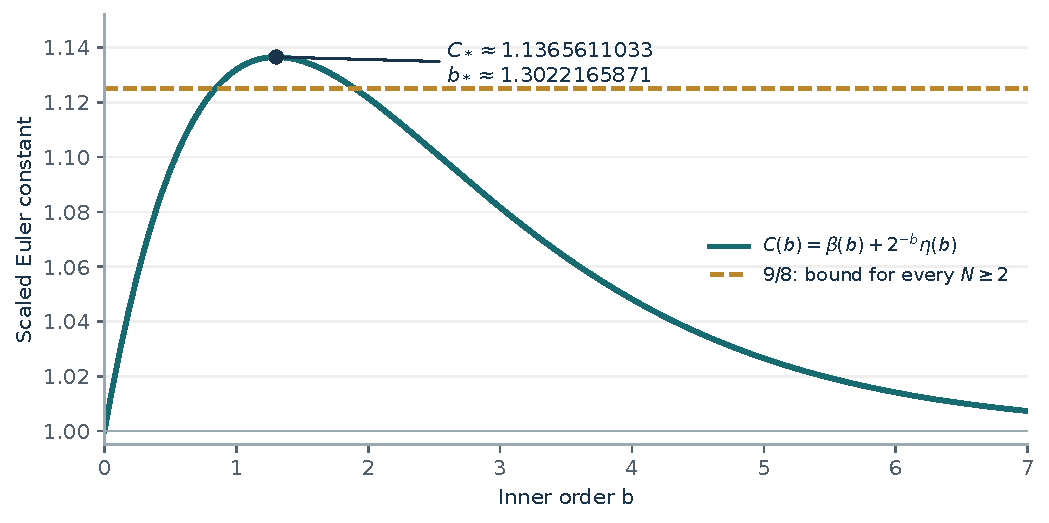
\includegraphics[width=.88\linewidth]{figures/euler_axis.pdf}
\caption{The inherited axis function and the new strict separator for
every later Euler step. The curve is a numerical illustration; the
maximum is defined exactly by \eqref{eul:eq:Cstar}, and the separation
from $9/8$ has the rational witness \eqref{eul:eq:C-lower}.}
\label{eul:fig:axis}
\end{figure}

\subsection{A probability representation with no threshold}

For $s>0$ let $\mu_s$ be the probability measure on $(0,1)$ with density
\begin{equation}\label{eul:eq:mu}
 d\mu_s(x)=\frac{(-\log x)^{s-1}}{\Gamma(s)}\,dx.
\end{equation}
Equivalently, $X_s=e^{-T_s}$ where $T_s$ is gamma distributed with
shape $s$ and rate one. The elementary gamma integral gives
\[
 \int_0^1x^{n-1}\,d\mu_s(x)=n^{-s}\qquad(n>0).
\]
At $s=0$, when needed, set $\mu_0=\delta_1$.

\begin{lemma}[Positive double integral]\label{eul:lem:positive}
For independent $X\sim\mu_a$ and $Y\sim\mu_b$,
\begin{align}
 A_k&=\E\!\left[X^{2k}\frac{1-Y^{2k}}{1-Y}\right],\label{eul:eq:moment}\\
 F_{a,b}(z)&=z^2\E\!\left[
       \frac{X}{(1-zX)(1-zXY)}\right]
       \qquad(z\in\C\setminus[1,\infty)).\label{eul:eq:F-integral}
\end{align}
In particular,
\begin{equation}\label{eul:eq:gaussian-integral}
 -g_{a,b}=\E\!\left[
 \frac{X^2(1+Y)}{(1+X^2)(1+X^2Y^2)}\right]>0.
\end{equation}
These formulas also hold for $a=0,b>0$.
\end{lemma}
\begin{proof}
Expand $(1-Y^m)/(1-Y)=\sum_{r=0}^{m-1}Y^r$ and apply the gamma
moment formula. This proves \eqref{eul:eq:moment}. For $|z|<1$, absolute
convergence permits summation of the two geometric series in
\[
 \E\!\left[\frac{z}{1-Y}
     \left\{\frac1{1-zX}-\frac1{1-zXY}\right\}\right].
\]
Their difference is exactly the integrand in \eqref{eul:eq:F-integral}.
On a compact subset of the slit plane, both denominators stay uniformly
away from zero for $X,Y\in[0,1]$. The probability integral is therefore
holomorphic there and supplies the asserted principal continuation.
At $z=i$, rationalization gives \eqref{eul:eq:gaussian-integral}.
No signed-moment existence theorem is required.
\end{proof}

\begin{lemma}[Exact positive Euler tail]\label{eul:lem:tail}
Set
\begin{equation}\label{eul:eq:W-K}
 W_N(x)=\frac{(1-x^2)^N}{1+x^2},\qquad
 \mathcal K_N(x,y)=\frac{W_N(xy)-W_N(x)}{1-y}.
\end{equation}
Then, for every $N\ge1$,
\begin{equation}\label{eul:eq:tail}
 2^N(E_N-g_{a,b})=\E[\mathcal K_N(X,Y)].
\end{equation}
The integrand is strictly positive for $0<x,y<1$.
\end{lemma}
\begin{proof}
Apply the binomial theorem to the finite expression in
\eqref{eul:eq:moment}:
\begin{equation}\label{eul:eq:negative-increments}
 d_j=\E\!\left[
 \frac{(1-X^2)^j-(1-X^2Y^2)^j}{1-Y}\right]<0\qquad(j\ge1).
\end{equation}
For $u,v\in[0,1]$ the inequality $|u^j-v^j|\le j|u-v|$ gives
$|d_j|\le2j$. Thus the Euler series converges absolutely, uniformly
under the probability integral. Summing it gives
\[
 \sum_{j\ge0}2^{-j-1}d_j
 =\E\!\left[\frac{(1+X^2)^{-1}-(1+X^2Y^2)^{-1}}{1-Y}\right]
 =g_{a,b}.
\]
Summing only the terms $j\ge N$ yields \eqref{eul:eq:tail}. Since
$W_N$ is strictly decreasing on $(0,1)$, the sign is strict. The same
argument works at $a=0$, because then $X=1$ while $0<Y<1$.
\end{proof}

The identity \eqref{eul:eq:tail} separates the uniform problem into
an elementary kernel inequality and a probability average. Its first
case is
\begin{equation}\label{eul:eq:K1}
 \mathcal K_1(x,y)=
 \frac{2x^2(1+y)}{(1+x^2)(1+x^2y^2)}.
\end{equation}
The behavior of the later kernels is sufficiently different that
their bounds cannot be inferred solely from the size of $g_{a,b}$.

\subsection{Three polynomial inequalities control every later tail}

\begin{lemma}[Uniform kernel gap]\label{eul:lem:kernel-gap}
For every integer $N\ge2$, $0\le x\le1$, and $0\le y<1$,
\begin{equation}\label{eul:eq:kernel-gap}
 0\le\mathcal K_N(x,y)<\frac98.
\end{equation}
The same upper bound holds at $y=1$ by the continuous limiting value.
\end{lemma}

We give the reduction and all finite premises of the proof. Put $u=x^2$.
For $N=2,3$, define the polynomial
\begin{align}\label{eul:eq:PN}
 P_N(u,y)={}&9(1+u)(1+uy^2)\\
 &-8\frac{(1-uy^2)^N(1+u)-(1-u)^N(1+uy^2)}{1-y}.\notag
\end{align}
The numerator vanishes at $y=1$, so the quotient is a polynomial.
Direct division gives
\begin{align}\label{eul:eq:P2}
 P_2={}&9+u(9y^2-24y-15)\notag\\
 &+u^2(8y^3+17y^2+8y+8)+8u^3(y^3+y^2),
\end{align}
and
\begin{align}\label{eul:eq:P3}
 P_3={}&9+u(9y^2-32y-23)
       +u^2(24y^3+33y^2+24y+24)\notag\\
 &+u^3(-8y^5-8y^4+16y^3+16y^2-8y-8)\notag\\
 &-8u^4(y^5+y^4+y^3+y^2).
\end{align}
Exact positive Bernstein expansions on dyadic boxes prove
$P_2>0$ and $P_3>0$ on the closed unit square. Since
\[
 \frac98-\mathcal K_N(x,y)
 =\frac{P_N(x^2,y)}{8(1+x^2)(1+x^2y^2)},
\]
these prove the first two cases of the kernel lemma.

For $N\ge4$, write
$w_N(t)=(1-t)^N/(1+t)$ for $0\le t\le1$. Every derivative has the
alternating sign appropriate to its order: Leibniz's formula is a
sum of products of two factors with that property. Also
$w_N^{(j)}(1)=0$ for $j=0,1,2,3$. Taylor's formula with integral
remainder consequently gives
\begin{equation}\label{eul:eq:mixture}
 w_N(t)=\int_{(0,1]}(1-t/s)_+^4\,d\sigma_N(s),
\end{equation}
where
\begin{equation}\label{eul:eq:mixture-measure}
 d\sigma_N(s)=\frac{-s^4w_N^{(5)}(s)}{24}\,ds
             +\frac{w_N^{(4)}(1)}{24}\,\delta_1(ds).
\end{equation}
It is a positive measure, and setting $t=0$ shows that its mass is
$w_N(0)=1$. The atom has mass $1/2$ for $N=4$ and is absent for
$N>4$. This elementary truncated-power representation is a special
case of the classical multiply monotone framework
\cite{Williamson,McNeilNeslehova}; here Taylor's formula proves exactly
the representation used, including its endpoint atom.

For fixed $0<y<1$, the largest value over $r\ge0$ of
\[
 \frac{(1-r^2y^2)_+^4-(1-r^2)_+^4}{1-y}
\]
occurs at
\[
 r^2=\frac{1-y^{2/3}}{1-y^{8/3}}<1.
\]
Indeed, in $0<r<1$ differentiation in $r^2$ gives this unique critical
point, with derivative positive before it and negative afterwards.
For $r\ge1$ the expression is decreasing until it becomes zero.
Its maximum is therefore
\begin{equation}\label{eul:eq:M4}
 M_4(y)=\frac{(1-y)^3(1+y)^4}{(1-y^{8/3})^3}.
\end{equation}
The limiting values at $y=0,1$ are also finite. Set $y=v^3$ and
define
\begin{equation}\label{eul:eq:Q4}
 Q_4(v)=\frac{9(1-v^8)^3-8(1-v^3)^3(1+v^3)^4}{(1-v)^3}.
\end{equation}
The expression is a polynomial of degree 21. Two exact Bernstein
expansions, on $[0,1/2]$ and $[1/2,1]$, have strictly positive
coefficients. Hence $M_4(y)<9/8$ for $0\le y<1$, and the limiting
case also satisfies the strict bound. Substitute \eqref{eul:eq:mixture}
into \eqref{eul:eq:W-K}, with $r=x/\sqrt{s}$. This ratio may exceed
one, which is why the preceding maximization included all $r\ge0$.
A probability average of quantities bounded by $M_4(y)$ proves
\eqref{eul:eq:kernel-gap} for all $N\ge4$.

\subsection{The finite positivity certificates}

For clarity, the proof certificate does not use a numerical polynomial
optimizer. If $p(t)=\sum_{j=0}^{d}a_jt^j$, its degree-$d$ Bernstein
coefficients on $[0,1]$ are
\begin{equation}\label{eul:eq:bernstein}
 b_k=\sum_{j=0}^{k}a_j\frac{\binom{k}{j}}{\binom{d}{j}},\qquad
 p(t)=\sum_{k=0}^{d}b_k\binom{d}{k}t^k(1-t)^{d-k}.
\end{equation}
The basis functions are nonnegative and sum to one. For a box in
several variables, first make an affine substitution to the unit box
and then apply the formula in each variable. Positivity of every
coefficient proves strict positivity on the whole closed box.

The standard-library verifier \src{code/certify_euler_bound.py}
constructs the three polynomials directly from
\eqref{eul:eq:PN} and \eqref{eul:eq:Q4}, checking each exact polynomial
division. It recursively bisects a box only when its current
Bernstein coefficients do not already prove positivity. The resulting
finite partition and its exact rational lower coefficients are written
to \src{data/euler_polynomial_certificate.json}.

\begin{center}
\begin{tabular}{@{}lrrl@{}}
\toprule
Polynomial & Boxes & Positive coefficients & Smallest coefficient\\
\midrule
$P_2$ & 13 & 208 & $3/64$\\
$P_3$ & 7 & 210 & $11337/40960$\\
$Q_4$ & 2 & 44 & $1$\\
\bottomrule
\end{tabular}
\end{center}

Thus the proof uses 462 positive rational coefficients in total.
An independent SymPy verifier reconstructs the expressions without
importing the producer's polynomial operations, checks all coefficients,
checks that box interiors are disjoint, and checks that their total
volume is one. The producer's recursive bisection already ensures
coverage; the independent checks also make the stored partition
directly reviewable.

\subsection{Why the first step determines the exact optimum}

For fixed $y\in(0,1)$, \eqref{eul:eq:K1} is strictly increasing in
$x\in(0,1)$, because its derivative has the positive factor
$1-x^4y^2$. Consequently
\begin{equation}\label{eul:eq:axis-domination}
 -2g_{a,b}=\E[\mathcal K_1(X,Y)]
 <\E\!\left[\frac{1+Y}{1+Y^2}\right]=C(b)
 \qquad(a>0).
\end{equation}
The equality on the right follows either from the axis formula
$F_{0,b}(z)=z\Li_b(z)/(1-z)$ or by the convergent residue-class
definitions of $\beta$ and $\eta$. As $a\downarrow0$, $X\to1$
in probability, so bounded convergence gives equality in the limit.

The following prerequisite was already proved in the baseline. We
include its principal argument to make the use of the maximum
self-contained.

\begin{proposition}[The inherited axis maximum]\label{eul:prop:axis}
The function $C$ in \eqref{eul:eq:Cstar} has exactly one stationary
point on $(0,\infty)$. It is a nondegenerate global maximum. Moreover,
$C(b)>1$ for finite $b>0$, and $C(b)\to1$ at both ends of the interval.
\end{proposition}
\begin{proof}
Let $\varphi(T)=(1+e^{-T})/(1+e^{-2T})$. Then
$C(b)=\E[\varphi(T_b)]$. The function $\varphi$ increases and then
decreases, its unique maximum being at $T=\log(1+\sqrt2)$.
It is larger than one and at most $(1+\sqrt2)/2$ for finite $T>0$.
Gamma concentration at zero as $b\downarrow0$, and at infinity as
$b\to\infty$, gives the endpoint limits and existence of a maximum.

For $1<\lambda<\max\varphi$, the function
$f(T)=\varphi(T)-\lambda$ has exactly two sign changes $T_1<T_2$,
with signs negative, positive, negative. It is impossible that
$C(b_j)=\lambda$ at three distinct $b_1<b_2<b_3$. To see this, put
$v=T^{b_2-b_1}$ and $p=(b_3-b_1)/(b_2-b_1)>1$.
Subtract from $v^p$ the secant line through its values at $T_1,T_2$,
and multiply by $-T^{b_1-1}$. Strict convexity produces a linear
combination of the three powers $T^{b_j-1}$ with the same strict
sign pattern as $f$. Its integral against $f(T)e^{-T}$ is positive,
contradicting the three vanishing Mellin integrals.

At a stationary point $b_0$, put $\lambda=C(b_0)$. If $C''(b_0)=0$
as well, the Mellin integral of $f$ and its first two derivatives in
$b$ vanish. Their linear combination with kernel
\[
 -T^{b_0-1}(\log T-\log T_1)(\log T-\log T_2)
\]
again gives a strictly positive integral, a contradiction. Every
stationary point is therefore nondegenerate. A local minimum would
give three intersections with its horizontal level, since the two
endpoint limits are lower; hence every stationary point is a strict
maximum. There can be only one. All differentiations are justified
by the exponential tail and integrable powers of $|\log T|$ at zero.
\end{proof}

The finer bracket $1<b_*<2$ is inherited from the baseline's exact
comparison at $b=3/2$ and its elementary endpoint bounds. The new
Euler theorem only needs uniqueness and $C_*>9/8$. Even that last
strict inequality has a very short independent rational witness:
\begin{equation}\label{eul:eq:C-lower}
 C_*\ge C(1)>-2E_8(0,1)
 =\frac{1627631}{1441440}>\frac98.
\end{equation}
The finite value uses rational harmonic numbers and
\eqref{eul:eq:definitions}; the strict first comparison follows from
the negative Euler increments. It is checked by the same exact script.

\begin{proof}[Proof of \cref{eul:thm:main}]
Absolute convergence, strict decrease, and the exact tail follow from
\cref{eul:lem:tail}. The kernel gap gives
\eqref{eul:eq:universal-nine-eighths}. For $N=1$, $E_1=0$, and
\eqref{eul:eq:axis-domination} bounds the scaled error by $C_*$.
For every $N\ge2$, \eqref{eul:eq:C-lower} makes the universal
$9/8$ bound strictly smaller than $C_*$. This proves
\eqref{eul:eq:sharp-universal}.

Fix $b=b_*$ and let $a\downarrow0$. At $N=1$ the scaled error
converges to $C_*$. No smaller universal constant is possible.
For $a=0$ equality is attained at $b=b_*$, $N=1$; uniqueness of
the axis maximum, strictness in \eqref{eul:eq:axis-domination}, and
the gap for $N\ge2$ exclude every other equality case.
\end{proof}

\subsection{Consequences for certified computation}

The new bound removes the parameter restrictions from the error
budget. Given an exact or outward-enclosed finite Euler sum with
$N\ge2$, the analytic Gaussian value lies in
\begin{equation}\label{eul:eq:certified-interval}
 E_N-\frac{9}{8\,2^N}<g_{a,b}<E_N.
\end{equation}
If the finite sum itself is enclosed by $[L_N,U_N]$, use
$[L_N-9/(8\,2^N),U_N]$. Fractional-power rounding errors must be
included in $[L_N,U_N]$; the theorem certifies truncation error only.
For a requested truncation tolerance $\varepsilon>0$, any
\[
 N\ge\max\!\left(2,\left\lceil
         \log_2\frac{9}{8\varepsilon}\right\rceil\right)
\]
suffices. No signed-kernel mass, parameter-dependent zeta bound,
or numerical estimate of $b_*$ enters this choice.

The finite binomial-tail formula from the baseline remains useful:
\begin{equation}\label{eul:eq:finite-weights}
 E_N=2^{-N}\sum_{k=0}^{N-1}(-1)^k A_k
                   \sum_{j=k+1}^{N}\binom Nj.
\end{equation}
It follows by interchanging the two finite sums in
\eqref{eul:eq:definitions} and applying Pascal's identity. Its
coefficients allow exact rational accumulation when the orders are
integers, and interval accumulation otherwise.

\begin{remark}[What remains unoptimized]
The number $9/8$ is a convenient certified separator, not a claim
of the least constant restricted to $N\ge2$. Numerically the
pointwise kernel maximum at $N=2$ is about $1.11894$, below $9/8$;
averaging against the gamma laws may lower the optimum further.
Neither observation is used in the proof. The all-$N$ optimum is
nevertheless exact because the first-step supremum is strictly larger
than the proved bound on every later step.
\end{remark}

\section{Exact certificates for the remaining golden weight-five ladders}
\label{gold:sec}

Put
\[
 \rho=\frac{\sqrt5-1}{2},\qquad \phi=\rho^{-1},\qquad
 \lambda=\log\rho=-\log\phi.
\]
The golden-ratio discussion in the audited manuscript identifies three
weight-five evaluations with the index-$12$, $20$, and $24$ ladder
families, and records numerical evidence for them \cite{Repo}.
The first evaluation has already received an analytic proof in the
preceding research.  The contribution here is a complete local proof
certificate for each of the other two evaluations, together with all
its lower-weight companions.  These are statements about what is now
proved explicitly in the repository's research program; they do not
assert historical priority for the ladder evaluations.  The general
connection between rational-function identities, tensor kernels, and
polylogarithm ladders is classical; see Gangl \cite{Gangl}.

The certificates use rational functions of one variable.  Consequently,
the lower-weight conclusions follow from identities holding on an open
interval.  No differentiation of an identity valid only at the isolated
algebraic number $\rho$ is involved.

\subsection{The two evaluations and their full descent}

Define two finitely supported coefficient vectors by
\begin{align}
 (c^{\mathrm{II}}_2,c^{\mathrm{II}}_4,c^{\mathrm{II}}_{10},
     c^{\mathrm{II}}_{20})&=(45000,-16875,-144,9),
 \label{gold:eq:cII}\\
 (c^{\mathrm{III}}_2,c^{\mathrm{III}}_4,c^{\mathrm{III}}_6,
     c^{\mathrm{III}}_8,c^{\mathrm{III}}_{24})
     &=(15660,-19440,7680,2430,-15).
 \label{gold:eq:cIII}
\end{align}
A missing coefficient means zero.  The superscripts refer to the
second and third displayed golden weight-five formulas in the
manuscript; the third vector is the displayed formula before the
canonical index-$24$ recombination.

\begin{theorem}[Golden evaluations with exact descent]
\label{gold:thm:main}
For either vector $c=c^{\mathrm{II}},c^{\mathrm{III}}$, put
\[
 S_m=\sum_{j\ge1}c_jj^{5-m}\Li_m(\rho^j),\qquad 1\le m\le5.
\]
Then
\begin{equation}
 S_m=\frac{a\lambda^m}{m!}
     +\sum_{r=2}^{m}q_r\zeta(r)\frac{\lambda^{m-r}}{(m-r)!},
 \label{gold:eq:all-weights}
\end{equation}
where the constants are
\begin{center}
\begin{tabular}{c|rrrrr}
 & $a$ & $q_2$ & $q_3$ & $q_4$ & $q_5$\\ \hline
 $\mathrm{II}$ & $720000$ & $-57600$ & $0$ & $32040$ & $28944$\\
 $\mathrm{III}$ & $-250560$ & $8640$ & $0$ & $2520$ & $5025$
\end{tabular}
\end{center}
In particular, writing $\ell=\log\phi$, the two weight-five evaluations are
\begin{align}
 &45000\Li_5(\rho^2)-16875\Li_5(\rho^4)
       -144\Li_5(\rho^{10})+9\Li_5(\rho^{20})\notag\\
 &\hspace{12mm}=28944\zeta(5)-6000\ell^5
           +1600\pi^2\ell^3-356\pi^4\ell,
 \label{gold:eq:II-five}\\[2mm]
 &15660\Li_5(\rho^2)-19440\Li_5(\rho^4)
       +7680\Li_5(\rho^6)+2430\Li_5(\rho^8)
       -15\Li_5(\rho^{24})\notag\\
 &\hspace{12mm}=5025\zeta(5)+2088\ell^5
          -240\pi^2\ell^3-28\pi^4\ell.
 \label{gold:eq:III-five}
\end{align}
\end{theorem}

The vanishing $q_3=0$ matters: the descent produces no
$\zeta(3)\lambda^2$ term at weight five.  This cancellation will follow
from the exact endpoint arithmetic of the functional certificates.

\subsection{A real generalized Rogers function}

For $n\ge2$ and real $x\ne0,1$, define
\begin{align}
 \mathcal R_n(x)
 &=\sum_{r=0}^{n-2}\frac{(-\log|x|)^r}{r!}
                  \operatorname{Re}\Li_{n-r}(x)\notag\\
 &\quad+\frac{(-1)^{n-1}(n-1)}{n!}
           \log^{n-1}|x|\operatorname{Re}\Li_1(x).
 \label{gold:eq:R-definition}
\end{align}
Here the ordinary polylogarithms use their principal branches, and
$\operatorname{Re}\Li_1(x)=-\log|1-x|$.  We extend the definition
continuously by $\mathcal R_n(0)=0$ and $\mathcal R_n(1)=\zeta(n)$.
The first functions are
\begin{align*}
 \mathcal R_2(x)&=\operatorname{Re}\Li_2(x)
                +\tfrac12\log|x|\log|1-x|,\\
 \mathcal R_3(x)&=\operatorname{Re}\Li_3(x)
                -\log|x|\operatorname{Re}\Li_2(x)
                -\tfrac13\log^2|x|\log|1-x|,\\
 \mathcal R_4(x)&=\operatorname{Re}\Li_4(x)
                -\log|x|\operatorname{Re}\Li_3(x)
                +\tfrac12\log^2|x|\operatorname{Re}\Li_2(x)
                -\tfrac18\log^3|x|\operatorname{Re}\Li_1(x),\\
 \mathcal R_5(x)&=\operatorname{Re}\Li_5(x)
                -\log|x|\operatorname{Re}\Li_4(x)
                +\tfrac12\log^2|x|\operatorname{Re}\Li_3(x)\\
 &\qquad-\tfrac16\log^3|x|\operatorname{Re}\Li_2(x)
                +\tfrac1{30}\log^4|x|\operatorname{Re}\Li_1(x).
\end{align*}
In particular, $\mathcal R_3$ is the usual real single-valued
trilogarithm.  At higher weights it is useful to retain
$\mathcal R_n$ itself, including at even weights.

\begin{lemma}[Derivative, inversion, and duplication]
\label{gold:lem:R}
Write $L=\log|x|$ and $M=\log|1-x|$.  On each real interval avoiding
$0$ and $1$,
\begin{equation}
 d\mathcal R_n(x)
   =\frac{(-1)^n(n-1)}{n!}
       L^{n-2}\bigl(L\,dM-M\,dL\bigr).
 \label{gold:eq:R-derivative}
\end{equation}
Let
\[
 h_n(+1)=1,\qquad h_n(-1)=-(1-2^{1-n}).
\]
For nonzero real $x$,
\begin{align}
 \mathcal R_n(x^{-1})
 &=(-1)^{n-1}\mathcal R_n(x)
   +\bigl(1-(-1)^{n-1}\bigr)h_n(\operatorname{sgn}x)\zeta(n),
 \label{gold:eq:R-inversion}\\
 \mathcal R_n(x)+\mathcal R_n(-x)
 &=2^{1-n}\mathcal R_n(x^2).
 \label{gold:eq:R-duplication}
\end{align}
\end{lemma}

\begin{proof}
The derivative relation
$d\operatorname{Re}\Li_j(x)=\operatorname{Re}\Li_{j-1}(x)\,dL$
holds for $j\ge2$.  Consequently the derivative of
\[
 F_n(x)=\sum_{r=0}^{n-1}\frac{(-L)^r}{r!}
                      \operatorname{Re}\Li_{n-r}(x)
\]
telescopes to $(-1)^nL^{n-1}dM/(n-1)!$.
Since
\[
 \mathcal R_n=F_n+\frac{(-1)^{n-1}}{n!}L^{n-1}M,
\]
one more differentiation proves \eqref{gold:eq:R-derivative}.
Under inversion, $(L,M)$ becomes $(-L,M-L)$.  Substitution in the
derivative formula shows that the difference in
\eqref{gold:eq:R-inversion} is constant separately on each of the
positive and negative half-axes.  Evaluation at $x=1$ and $x=-1$
fixes the constants, because
\[
 \mathcal R_n(-1)=\Li_n(-1)=-(1-2^{1-n})\zeta(n).
\]
The duplication formula follows term by term from the ordinary
polylogarithm duplication formula and $\log(x^2)=2\log|x|$.
These arguments extend across $x=1$ by continuity.  In
\eqref{gold:eq:R-definition}, the potentially singular monologarithm
is multiplied by a positive power of $\log|x|$, and its product tends
to zero as $x\to1$.
\end{proof}

\subsection{A tensor certificate with an elementary analytic interpretation}

Let $V=\mathbb Q(t)^\times\otimes_{\mathbb Z}\mathbb Q$, with the
multiplicative group written additively.  Signs are torsion and therefore
vanish in $V$.  For a nonzero rational function $f\ne1$, put
\[
 \beta_n[f]=f^{\otimes(n-2)}\otimes\bigl(f\wedge(1-f)\bigr).
\]
The repeated first factors can equivalently be placed in a symmetric
tensor power.  Only elementary linear algebra with this notation is
needed below.

The rational functions in the certificates have the form
\begin{equation}
 f_{s,a,b,c}(t)=s\,t^a(1-t)^b(1+t)^c,
 \qquad s\in\{1,-1\}.
 \label{gold:eq:arguments}
\end{equation}
They have neither zeros nor poles for $0<t<1$.  Define
\begin{equation}
 k(a,b,c)=a+2b-c.
 \label{gold:eq:k}
\end{equation}
This integer is the exponent after golden specialization, since
$1-\rho=\rho^2$ and $1+\rho=\rho^{-1}$.

\begin{lemma}[Exact descent from a rational-function certificate]
\label{gold:lem:descent}
Suppose $f_i=f_{s_i,a_i,b_i,c_i}$ and $u_i\in\mathbb Q$ satisfy
\begin{equation}
 \sum_i u_i\beta_5[f_i]=0.
 \label{gold:eq:tensor-certificate}
\end{equation}
Write $k_i=a_i+2b_i-c_i$.  For $2\le n\le5$, the function
\begin{equation}
 H_n(t)=\sum_i u_i k_i^{5-n}\mathcal R_n(f_i(t))
 \label{gold:eq:functional-family}
\end{equation}
is constant on $0<t<1$.  If all $a_i\ge0$, its value is
\begin{equation}
 H_n(t)=E_n\zeta(n),\qquad
 E_n=\sum_{a_i=0}u_i k_i^{5-n}h_n(s_i).
 \label{gold:eq:E}
\end{equation}
We use $k_i^0=1$, including when $k_i=0$.
\end{lemma}

\begin{proof}
Extend the assignments
\[
 \eta(t)=1,\qquad \eta(1-t)=2,\qquad \eta(1+t)=-1
\]
to a linear functional $\eta:V\to\mathbb Q$.  For example, assign
zero to every other primitive irreducible polynomial and every rational
prime.  Then $\eta(f_i)=k_i$.  Contracting $5-n$ of the first three
tensor factors in \eqref{gold:eq:tensor-certificate} gives
\begin{equation}
 \sum_i u_i k_i^{5-n}\beta_n[f_i]=0.
 \label{gold:eq:contracted}
\end{equation}
For a fixed regular $t$, evaluate a tensor factor $g$ by $\log|g(t)|$,
and evaluate a wedge $g\wedge h$ by
\[
 \log|g(t)|\,d\log|h(t)|
 -\log|h(t)|\,d\log|g(t)|.
\]
Equation \eqref{gold:eq:contracted}, together with
\eqref{gold:eq:R-derivative}, gives $dH_n=0$.
There are only finitely many points in $(0,1)$ where some $f_i(t)=1$.
The functions $\mathcal R_n(f_i(t))$ are continuous at these points,
so the constants on the intervening intervals agree.
Finally, if $a_i>0$ then $f_i(t)\to0$ as $t\to0^+$, while if
$a_i=0$ then $f_i(t)\to s_i$.  These limits prove \eqref{gold:eq:E}.
\end{proof}

A rational constant in $1-f_i$ must be retained when verifying the
tensor equation.  For example,
\[
 1-\frac{1-t}{1+t}=\frac{2t}{1+t}
\]
contributes the independent constant-prime coordinate $2$ to $1-f_i$.
It has logarithm $\log2$ and derivative zero; discarding it would change
both the tensor equation and its analytic interpretation.  The
certificates below and the verification program retain this coordinate.

\subsection{The two finite certificates}

Table~\ref{gold:tab:certificates} defines coefficients $u_{s,a,b,c}$
and $v_{s,a,b,c}$.  An entry $0$ means that the corresponding argument
is absent.  There are $58$ nonzero $u$ entries and $60$ nonzero $v$
entries.  For each column separately,
\begin{equation}
 \sum_{s,a,b,c}u_{s,a,b,c}\beta_5[f_{s,a,b,c}]=0,
 \qquad
 \sum_{s,a,b,c}v_{s,a,b,c}\beta_5[f_{s,a,b,c}]=0.
 \label{gold:eq:two-certificates}
\end{equation}
Thus the table also gives two explicit rational-function identities
\eqref{gold:eq:functional-family}, and four weights of each identity.
Their endpoint constants are displayed below.

Here is a completely finite interpretation of the two checks in
\eqref{gold:eq:two-certificates}.  Factor every $f$ and $1-f$ over
$\mathbb Q(t)$, including the rational contents.  Use rational primes
and primitive irreducible polynomials as a multiplicative basis modulo
signs.  Write the factor vectors as $e_f$ and $d_f$.  For each unordered
pair of basis indices $(p,q)$ and each triple $(i,j,k)$ chosen with
repetition from the three coordinates $t,1-t,1+t$, verify
\begin{equation}
 \sum_f u_f(e_f)_i(e_f)_j(e_f)_k
 \bigl((e_f)_p(d_f)_q-(e_f)_q(d_f)_p\bigr)=0,
 \label{gold:eq:finite-coordinate-check}
\end{equation}
and then the same equation with $u$ replaced by $v$.
The first column has $16$ basis coordinates, including the prime $2$;
the second has $18$, also including $2$.  There are respectively
$330$ and $370$ potentially nonzero weight-five coordinate sums, and
every one is zero.  These are exact integer equalities.
The supplied verifier factors the functions afresh and performs these
sums using rational arithmetic.  It additionally checks all four
contracted tensor equations directly.

\begingroup
\small
\setlength{\tabcolsep}{9pt}
\begin{longtable}{rrrrrr}
\caption{The two weight-five rational-function certificates.  The
argument in a row is $s\,t^a(1-t)^b(1+t)^c$.}
\label{gold:tab:certificates}\\
\hline
$s$&$a$&$b$&$c$&$u$&$v$\\ \hline
\endfirsthead
\multicolumn{6}{c}{Table~\ref{gold:tab:certificates} continued}\\
\hline $s$&$a$&$b$&$c$&$u$&$v$\\ \hline
\endhead
\hline
\endfoot
1&0&0&1&-2166&-1161\\
-1&0&0&1&-3240&-2025\\
-1&0&0&3&40&25\\
1&0&1&-1&-80&-288\\
-1&0&1&-1&-80&-288\\
1&0&1&0&2178&3510\\
-1&0&1&0&2916&4536\\
1&0&1&1&6&-270\\
1&0&1&2&26&72\\
-1&0&2&-2&10&36\\
1&0&2&1&-54&-27\\
-1&0&3&0&-36&-56\\
-1&1&-3&-2&8&9\\
1&1&-2&-3&-4&-9\\
-1&1&-2&-1&-40&0\\
-1&1&-2&0&284&405\\
1&1&-1&-1&-6&27\\
-1&1&-1&-1&-162&-351\\
1&1&-1&0&2268&2997\\
-1&1&-1&0&1722&2430\\
-1&1&-1&1&-105&-360\\
1&1&0&-2&-320&-144\\
1&1&0&-1&-1710&-81\\
-1&1&0&-1&-2592&-486\\
1&1&0&0&-1236&-54\\
-1&1&0&0&528&1539\\
1&1&0&1&-126&-414\\
-1&1&0&1&-480&-405\\
1&1&1&-1&-70&-270\\
1&1&1&0&444&909\\
-1&1&1&0&-42&9\\
1&1&1&1&-72&-81\\
-1&1&1&1&42&81\\
-1&1&2&1&0&9\\
-1&1&3&1&5&0\\
-1&2&-2&-1&-72&-81\\
-1&2&-1&-2&32&81\\
-1&2&-1&-1&6&-270\\
1&2&-1&0&-206&-504\\
-1&2&-1&0&204&234\\
1&2&0&-1&38&99\\
-1&2&0&-1&-240&270\\
-1&2&0&0&-210&-540\\
1&2&1&0&-60&0\\
-1&2&1&0&0&81\\
1&3&-3&-3&0&-1\\
1&3&-3&0&-28&-37\\
1&3&-2&-1&-46&-9\\
-1&3&-1&-2&18&54\\
-1&3&-1&-1&-30&0\\
-1&3&-1&0&-72&-81\\
1&3&-1&1&14&45\\
-1&3&0&-3&32&6\\
1&3&0&-1&12&81\\
-1&3&0&-1&0&81\\
-1&3&0&0&4&19\\
1&4&-3&-2&4&0\\
-1&4&-1&-2&0&9\\
-1&4&0&1&8&9\\
-1&4&1&0&-8&-9\\
1&5&-3&-1&8&9\\
-1&5&-1&-3&-3&-9\\
1&5&1&-1&0&9\\
-1&6&3&0&0&-1\\
-1&7&1&-1&1&0\\
-1&9&0&-3&0&-1\\
\end{longtable}
\endgroup

The table was obtained by exact linear algebra on the functions
\eqref{gold:eq:arguments} with numerator and denominator degrees at most
$9$, after cancellation of common factors.  The search discovers the
rows; the explicit table and the coordinate equations
\eqref{gold:eq:finite-coordinate-check} are the proof certificate.
A complete classification of all functional identities in this or a
larger alphabet is not needed for the argument.

\subsection{Golden specialization and the endpoint constants}

At $t=\rho$, the table argument becomes $s\rho^k$, with
$k=a+2b-c$.  Applying inversion to negative exponents and duplication
to negative arguments gives
\begin{align}
 \sum_f u_f k_f^{5-n}\mathcal R_n(f(\rho))
 &=\frac1{144}\sum_{j\ge1}c^{\mathrm{II}}_j
           j^{5-n}\mathcal R_n(\rho^j)
      +B_n^{\mathrm{II}}\zeta(n),
 \label{gold:eq:u-image}\\
 \sum_f v_f k_f^{5-n}\mathcal R_n(f(\rho))
 &=\frac1{120}\sum_{j\ge1}c^{\mathrm{III}}_j
           j^{5-n}\mathcal R_n(\rho^j)
      +B_n^{\mathrm{III}}\zeta(n).
 \label{gold:eq:v-image}
\end{align}
The constant $B_n$ includes the inversion constants at even weights
and any terms with $k=0$ at weight five.  All remaining coefficients
in \eqref{gold:eq:u-image}--\eqref{gold:eq:v-image} are exact rational
row sums.  The boundary computation is
\begin{center}
\small
\begin{tabular}{c|rrr|rrr}
 &\multicolumn{3}{c|}{$u$ column}&\multicolumn{3}{c}{$v$ column}\\
$n$&$E_n$&$B_n$&$E_n-B_n$&$E_n$&$B_n$&$E_n-B_n$\\ \hline
2&$7122$&$7522$&$-400$&$7695$&$7623$&$72$\\
3&$0$&$0$&$0$&$0$&$0$&$0$\\
4&$-2721/2$&$-1583$&$445/2$&$-7269/4$&$-7353/4$&$21$\\
5&$2205/8$&$597/8$&$201$&$-1011/4$&$-2357/8$&$335/8$
\end{tabular}
\end{center}
For example, the weight-five rational-function identities themselves are
\begin{equation}
 \sum_f u_f\mathcal R_5(f(t))=\frac{2205}{8}\zeta(5),\qquad
 \sum_f v_f\mathcal R_5(f(t))=-\frac{1011}{4}\zeta(5),
 \quad 0<t<1.
 \label{gold:eq:new-functional-identities}
\end{equation}
The golden power with exponent zero contributes $597\zeta(5)/8$ in
the first specialization and $-2357\zeta(5)/8$ in the second.
Subtracting these terms gives $201\zeta(5)$ and
$335\zeta(5)/8$, respectively.  Multiplication by $144$ and $120$
therefore gives the weight-five constants $28944$ and $5025$.

For transparency, the power and sign bookkeeping in every weight can
be expressed without any polylogarithm manipulation.  A row of
coefficient $w$ has weighted coefficient $w k^{5-n}$.  If $k<0$ and
$n$ is even, add $2wk^{5-n}h_n(s)$ to $B_n$ and negate the remaining
coefficient.  Replace $k$ by $|k|$.  If $s=-1$, replace its remaining
coefficient $z$ at $-\rho^k$ by $-z$ at $\rho^k$ and
$2^{1-n}z$ at $\rho^{2k}$.  If $k=0$, put the resulting constant into
$B_n$.  This finite procedure gives every entry above.
Consequently
\begin{equation}
 \sum_{j\ge1}c_jj^{5-n}\mathcal R_n(\rho^j)=q_n\zeta(n),
 \qquad 2\le n\le5,
 \label{gold:eq:golden-R}
\end{equation}
with the constants stated in Theorem~\ref{gold:thm:main}.

\subsection{Removing the lower polylogarithms}

The weight-one companion can be computed using the following elementary
factorizations.  Each equality follows by reduction modulo
$\rho^2+\rho-1=0$, with $\sqrt5=2\rho+1$:
\begin{center}
\begin{tabular}{c|l@{\qquad}c|l}
$j$&$1-\rho^j$&$j$&$1-\rho^j$\\ \hline
$2$&$\rho$&$10$&$11\rho^5$\\
$4$&$\sqrt5\rho^2$&$12$&$8\sqrt5\rho^6$\\
$6$&$4\rho^3$&$20$&$55\sqrt5\rho^{10}$\\
$8$&$3\sqrt5\rho^4$&$24$&$144\sqrt5\rho^{12}$
\end{tabular}
\end{center}
For either vector $c$, the coefficients of $\log2$, $\log3$,
$\log5$, and $\log11$ in
$\sum_j c_jj^4\log(1-\rho^j)$ vanish.  Hence
\begin{equation}
 S_1=-\sum_jc_jj^4\log(1-\rho^j)
     =-\frac12\sum_jc_jj^5\lambda=a\lambda.
 \label{gold:eq:S1}
\end{equation}
The two sums $\sum_j c_jj^5$ are $-1440000$ and $501120$,
which give $a=720000$ and $a=-250560$.

\begin{proof}[Proof of Theorem~\ref{gold:thm:main}]
The finite polynomial identities \eqref{gold:eq:two-certificates},
Lemma~\ref{gold:lem:descent}, and the exact specialization arithmetic
prove \eqref{gold:eq:golden-R}.  Expand the definition of
$\mathcal R_n$ at $\rho^j$.  Since $\log(\rho^j)=j\lambda$, it gives
\begin{equation}
 q_n\zeta(n)=
 \sum_{r=0}^{n-2}\frac{(-\lambda)^r}{r!}S_{n-r}
 +\frac{(-1)^{n-1}(n-1)}{n!}\lambda^{n-1}S_1.
 \label{gold:eq:triangular}
\end{equation}
Starting with \eqref{gold:eq:S1}, this triangular system has the unique
solution \eqref{gold:eq:all-weights}.  One may also verify the formula
by substitution: the coefficients of each $q_j\zeta(j)$ reduce to
\[
 \sum_{r=0}^{n-j}\frac{(-1)^r}{r!(n-j-r)!}
   =\begin{cases}1,&j=n,\\0,&j<n,\end{cases}
\]
and the $a$ term cancels because
\[
 \sum_{r=0}^{n-2}\frac{(-1)^r}{r!(n-r)!}
   +\frac{(-1)^{n-1}(n-1)}{n!}=0.
\]
This proves all five weights.  Substituting
$\zeta(2)=\pi^2/6$, $\zeta(4)=\pi^4/90$, and $\lambda=-\ell$ in
the case $n=5$ proves the two asserted evaluations.
\end{proof}

Some useful lower-weight consequences, written with smaller integer
coefficient vectors, are
\begin{align}
 5\Li_2(\rho^2)-15\Li_2(\rho^4)-2\Li_2(\rho^{10})
    +\Li_2(\rho^{20})
 &=5\lambda^2-\frac{2\pi^2}{15},
 \label{gold:eq:II-two}\\
 50\Li_3(\rho^2)-75\Li_3(\rho^4)-4\Li_3(\rho^{10})
    +\Li_3(\rho^{20})
 &=\frac{100\lambda^3-8\pi^2\lambda}{3},
 \label{gold:eq:II-three}\\
 500\Li_4(\rho^2)-375\Li_4(\rho^4)-8\Li_4(\rho^{10})
    +\Li_4(\rho^{20})
 &=\frac{500\lambda^4}{3}-\frac{80\pi^2\lambda^2}{3}
    +\frac{89\pi^4}{45}.
 \label{gold:eq:II-four}
\end{align}
For the third displayed ladder one obtains
\begin{align}
 &87\Li_2(\rho^2)-864\Li_2(\rho^4)+1152\Li_2(\rho^6)
       +864\Li_2(\rho^8)-144\Li_2(\rho^{24})
    =\pi^2-87\lambda^2,
 \label{gold:eq:III-two}\\
 &87\Li_3(\rho^2)-432\Li_3(\rho^4)+384\Li_3(\rho^6)
       +216\Li_3(\rho^8)-12\Li_3(\rho^{24})\notag\\
 &\hspace{25mm}=-58\lambda^3+2\pi^2\lambda,
 \label{gold:eq:III-three}\\
 &87\Li_4(\rho^2)-216\Li_4(\rho^4)+128\Li_4(\rho^6)
       +54\Li_4(\rho^8)-\Li_4(\rho^{24})\notag\\
 &\hspace{25mm}=-29\lambda^4+2\pi^2\lambda^2+\frac{7\pi^4}{90}.
 \label{gold:eq:III-four}
\end{align}
These companions are exact consequences of the same certificate, with
no separate recognition of numerical constants.

\subsection{The first ladder and canonical normalization}

The first golden formula is included in the supplied replay data as a
small consistency and normalization certificate.  Its ordinary
coefficient vector is
\[
 (c^{\mathrm I}_2,c^{\mathrm I}_4,c^{\mathrm I}_6,c^{\mathrm I}_{12})
       =(4455,-1215,-360,15).
\]
A primitive functional certificate has the following twelve rows in
the notation \eqref{gold:eq:arguments}:
\begin{center}
\small
\begin{tabular}{rrrr|r@{\qquad}rrrr|r}
$s$&$a$&$b$&$c$&$w$&$s$&$a$&$b$&$c$&$w$\\ \hline
$1$&$0$&$0$&$1$&$-54$&$1$&$1$&$0$&$0$&$-81$\\
$-1$&$0$&$0$&$1$&$-81$&$-1$&$1$&$0$&$0$&$-54$\\
$-1$&$0$&$0$&$3$&$1$&$-1$&$1$&$0$&$1$&$-9$\\
$1$&$1$&$0$&$-2$&$-9$&$-1$&$2$&$0$&$-1$&$-9$\\
$1$&$1$&$0$&$-1$&$-54$&$-1$&$3$&$0$&$-3$&$1$\\
$-1$&$1$&$0$&$-1$&$-81$&$1$&$3$&$0$&$0$&$1$
\end{tabular}
\end{center}
Its scale factor is $240$.  The same calculation gives
\[
 (a,q_2,q_3,q_4,q_5)=(84240,-6480,0,3420,3015),
\]
recovering the previously proved first evaluation.

For completeness, define the manuscript's canonical ladders explicitly.
For $N\in\{12,20,24\}$, write
\[
 T_N(m)=D_{N,1}\frac{\lambda^m}{m!}
       +D_{N,2}\zeta(2)\frac{\lambda^{m-2}}{(m-2)!}
       +D_{N,3}\zeta(4)\frac{\lambda^{m-4}}{(m-4)!},
\]
with any term having a negative factorial index omitted, and put
\begin{align*}
 L_{12}(m)&=\frac{\Li_m(\rho^{12})}{12^{m-1}}
 -\frac32\frac{\Li_m(\rho^6)}{6^{m-1}}
 -\frac{\Li_m(\rho^4)}{4^{m-1}}
 +\frac{11}{48}\frac{\Li_m(\rho^2)}{2^{m-1}}+T_{12}(m),\\
 L_{20}(m)&=\frac{\Li_m(\rho^{20})}{20^{m-1}}
 -\frac{\Li_m(\rho^{10})}{10^{m-1}}
 -3\frac{\Li_m(\rho^4)}{4^{m-1}}
 +\frac12\frac{\Li_m(\rho^2)}{2^{m-1}}+T_{20}(m),\\
 L_{24}(m)&=\frac{\Li_m(\rho^{24})}{24^{m-1}}
 -\frac43\frac{\Li_m(\rho^{12})}{12^{m-1}}
 -2\frac{\Li_m(\rho^8)}{8^{m-1}}\\
 &\quad+\frac73\frac{\Li_m(\rho^4)}{4^{m-1}}
 -\frac{205}{576}\frac{\Li_m(\rho^2)}{2^{m-1}}+T_{24}(m).
\end{align*}
The correction coefficients are
\[
\begin{array}{c|rrr}
 N&D_{N,1}&D_{N,2}&D_{N,3}\\ \hline
 12&-13/48&1/48&-19/1728\\
 20&-1/2&1/25&-89/4000\\
 24&179/576&-5/192&629/41472
\end{array}
\]
With these definitions, exact equality holds in
\[
 L_{12}(5)=\frac{67}{6912}\zeta(5),\qquad
 L_{20}(5)=\frac{201}{10000}\zeta(5),\qquad
 L_{24}(5)=-\frac{1541}{110592}\zeta(5).
\]
For the last value, add $64/3$ times the first ordinary weight-five
formula to the third, and divide by $-15\cdot24^4$; this eliminates
$\Li_5(\rho^6)$ and gives the manuscript's canonical index-$24$
combination.  The corresponding normalized first-degree ladders vanish
at weights $1,2,3,4$.  These statements follow by exact rational
recombination of \eqref{gold:eq:all-weights} and its first-ladder
counterpart.

\subsection{Verification, integration, and further questions}

The files \texttt{golden\_rational\_certificates.json} and
\texttt{certify\_golden\_ladders.py} contain the complete finite data and
an independent replay of the polynomial checks.  The verifier uses
SymPy to factor every rational function, retains rational-prime
coordinates, checks the tensor equations directly in all four weights,
performs every golden specialization, and checks the eight elementary
factorizations used for $S_1$.  Its separate $85$-digit calculations
verify the rational-function identities at $t=37/100$ and the ordinary
companions at $\rho$; these numerical diagnostics do not enter the proof.
The detailed receipt is
\texttt{golden\_certificate\_verification.json}.

For manuscript integration, the second and third displayed weight-five
formulas can be marked proved and linked to this section.  Their
first-degree lower-weight vanishing and the canonical values just
displayed can be marked proved as well.  The weight-$6$ through
weight-$9$ reconstructions have a different status: the present
certificates establish no upward continuation beyond weight five.
The contraction in Lemma~\ref{gold:lem:descent} decreases weight;
there is no inverse contraction that would produce the missing higher
functional identity.

Several follow-up questions are concrete.  First, can the $58$- and
$60$-term certificates be decomposed into a short list of named Kummer
specializations, giving a smaller human derivation?  Second, can a
larger rational-function alphabet produce the manuscript's weight-$6$
and weight-$7$ golden identities with similarly complete endpoint
bookkeeping?  Third, which part of the golden relation space is obtained
from a prescribed degree bound, and can exact matrix-rank certificates
prove useful minimality statements within that finite search model?
Fourth, the rational-function identities
\eqref{gold:eq:new-functional-identities} can be specialized at other
algebraic values satisfying multiplicative relations among
$t,1-t,1+t$; determining when their descended constants close on a
small polylogarithm basket is a systematic route to additional ladders.

\section{A certified double radial turning-point bifurcation}
\label{turn:sec:main}

The local radial problem has a second layer of degeneracy.  The
manuscript proves that the first nonconstant coefficient of the
normalized radius changes sign at a unique outer-order threshold for
each inner order $0<b<1$.  It subsequently proves opposite signs of the
next coefficient at two points of that threshold curve, and locates a
possible transition numerically \cite{Repo}.  Its final question in
\texttt{05-real-turning.tex} asks for the higher-order behavior at such a
transition.  We certify one transition, determine its next coefficient,
and prove that nearby normalized-radius curves can have two small-radius
turning points: a minimum followed by a maximum.

The conclusion is local in both the parameters and the radius.  It
does not settle the number of quartic transitions over the entire
interval $0<b<1$, nor exclude additional turning points farther from
the origin.  These distinctions matter because an initial Taylor
coefficient, even with a proved sign, does not control the whole disk.

\subsection{An exact finite recurrence to every radial order}
\label{turn:sec:recurrence}

For $a,b>0$, put
\begin{equation}
 F_{a,b}(z)=\sum_{n=2}^{\infty}p_n(a,b)z^n,
 \qquad
 p_n(a,b)=\frac{H_{n-1}^{(b)}}{n^a},
 \qquad
 H_{n-1}^{(b)}=\sum_{j=1}^{n-1}j^{-b}.
 \label{turn:eq:def}
\end{equation}
Let $\theta_{a,b}(\rho)$ denote the local solution near $\pi/2$ of
\[
 \operatorname{Im}F_{a,b}(\rho e^{i\theta})=0,
\]
for positive sufficiently small $\rho$, and set
\begin{equation}
 \eta_{a,b}(\rho)=\frac{\cos\theta_{a,b}(\rho)}{\rho},
 \qquad t=\rho^2.
 \label{turn:eq:eta}
\end{equation}
The radius $\rho$ in this section is a disk radius.  We write the
analytic extension in the squared radius as
$\eta_{a,b}(\rho)=\Phi(a,b,t)$.

\begin{proposition}[An all-orders finite coefficient identity]
\label{turn:prop:recurrence}
For $m\ge0$, define the polynomial
\begin{equation}
 E_m(y)=\sum_{n=m+2}^{2m+3}
  (-1)^{n-m-2}\binom{m+1}{n-m-2}
  2^{2m+3-n}p_n y^{2m+3-n}.
 \label{turn:eq:Em}
\end{equation}
Locally in $(a,b,t)$, the normalized-radius equation is the convergent
analytic identity
\begin{equation}
 \sum_{m=0}^{\infty}t^mE_m\bigl(\Phi(a,b,t)\bigr)=0.
 \label{turn:eq:implicit}
\end{equation}
There is a unique local analytic solution with
$\Phi(a,b,0)=\mu:=p_3/(2p_2)$.  If
\[
 \Phi(a,b,t)=\mu+\sum_{j\ge1}c_j(a,b)t^j,
\]
then the exact recursive identity is
\begin{equation}
 c_j=-\frac{1}{2p_2}[t^j]
 \sum_{m=1}^{j}t^m E_m\left(
   \mu+\sum_{\ell=1}^{j-1}c_\ell t^\ell\right).
 \label{turn:eq:coefficient-recursion}
\end{equation}
In particular, $c_j$ depends only on $p_2,\ldots,p_{2j+3}$.
\end{proposition}

\begin{proof}
For $\theta$ near $\pi/2$, divide the imaginary-part equation by
$\rho^3\sin\theta$ and use
$\sin(n\theta)=\sin\theta\,U_{n-1}(\cos\theta)$.  The finite Chebyshev
identity is
\[
 U_{n-1}(x)=\sum_{h=0}^{\lfloor(n-1)/2\rfloor}
  (-1)^h\binom{n-1-h}{h}(2x)^{n-1-2h}.
\]
After substituting $x=\rho y$, a summand in
$p_n\rho^{n-3}U_{n-1}(\rho y)$ has radius exponent
$2n-4-2h$.  It contributes to $t^m$ exactly when $h=n-2-m$.
The inequalities $0\le h\le\lfloor(n-1)/2\rfloor$ are equivalent to
$m+2\le n\le2m+3$.  Substitution gives precisely
\eqref{turn:eq:Em}.

This is an analytic identity, not merely a formal rearrangement.
On a compact complex neighborhood of fixed positive $(a,b)$, the
coefficients $p_n(a,b)$ are analytic and grow at most polynomially in
$n$.  The Chebyshev recurrence bounds $U_{n-1}(\rho y)$ exponentially
in $n$, uniformly when $y$ stays bounded and $\rho$ is sufficiently
small.  Hence the normalized series converges locally uniformly.  The
apparent negative power in its $n=2$ term cancels, leaving $2p_2y$;
all remaining powers of $\rho$ are nonnegative and even.  The sum is
therefore jointly analytic in $(a,b,t,y)$.

Now $E_0(y)=2p_2y-p_3$, and $2p_2\ne0$ at real positive parameters.
The analytic implicit-function theorem gives the unique solution
$y=\Phi(a,b,t)$ through $\mu=p_3/(2p_2)$.  For small positive $\rho$,
the angle $\arccos(\rho\Phi(a,b,\rho^2))$ is near $\pi/2$ and solves
the original equation, proving the claimed local interpretation.
Finally, the contribution of $E_0$ to the coefficient of $t^j$ is
$2p_2c_j$.  Since every other term has a factor $t^m$ with $m\ge1$,
its coefficient of degree $j$ uses only the already determined
$c_1,\ldots,c_{j-1}$.  Solving for $c_j$ proves
\eqref{turn:eq:coefficient-recursion}.
\end{proof}

The recurrence makes the finite nature of a local degeneracy test
explicit.  For example, no coefficient of $F_{a,b}$ beyond $p_9$ is
needed to determine the first three nonconstant coefficients of
$\eta$.  This is useful when a small coefficient results from nearly
cancelling terms: one can certify a finite expression directly instead
of estimating derivatives from values of the full boundary function.

\subsection{The sextic coefficient}
\label{turn:sec:sextic}

Write
\begin{equation}
 \Phi(a,b,t)=\mu+Kt+Qt^2+Rt^3+O(t^4).
 \label{turn:eq:expansion}
\end{equation}
Thus $K,Q,R$ are respectively the coefficients of
$\rho^2,\rho^4,\rho^6$ in the normalized radius.  Define
\begin{align}
 A(y)&=4p_3y^2-4p_4y+p_5,\notag\\
 B(y)&=8p_4y^3-12p_5y^2+6p_6y-p_7,\notag\\
 C(y)&=16p_5y^4-32p_6y^3+24p_7y^2-8p_8y+p_9.
 \label{turn:eq:ABC}
\end{align}
These are $E_1,E_2,E_3$ in Proposition~\ref{turn:prop:recurrence}.

\begin{proposition}[The first three nonconstant coefficients]
\label{turn:prop:sextic}
The exact coefficient formulas are
\begin{align}
 K&=-\frac{A(\mu)}{2p_2},\notag\\
 Q&=-\frac{A'(\mu)K+B(\mu)}{2p_2},\notag\\
 R&=-\frac{A'(\mu)Q+4p_3K^2+B'(\mu)K+C(\mu)}{2p_2}.
 \label{turn:eq:KQR}
\end{align}
At any simultaneous zero of $K$ and $Q$,
\begin{equation}
 R=-\frac{C(\mu)}{2p_2}.
 \label{turn:eq:Rzero}
\end{equation}
All these quantities are real analytic in positive $(a,b)$.
\end{proposition}

\begin{proof}
Retaining degrees at most three in \eqref{turn:eq:implicit} gives
\[
 0=2p_2\Phi-p_3+tA(\Phi)+t^2B(\Phi)+t^3C(\Phi)+O(t^4).
\]
The coefficients of $t,t^2,t^3$ are respectively
\begin{align*}
 &2p_2K+A(\mu),\\
 &2p_2Q+A'(\mu)K+B(\mu),\\
 &2p_2R+A'(\mu)Q+\tfrac12A''(\mu)K^2+B'(\mu)K+C(\mu).
\end{align*}
Since $A''=8p_3$, their vanishing gives
\eqref{turn:eq:KQR}.  The denominators do not vanish at positive
parameters, so analyticity follows from the finite formulas.
\end{proof}

The manuscript already identifies $K$ and $Q$ and proves that, on
the curve $K=0$, the quartic coefficient has opposite signs at
$b=1/2$ and $b=999/1000$.  The sextic formula supplies the missing
test when both of those earlier coefficients vanish.

\subsection{A unique certified transition in a rational rectangle}
\label{turn:sec:certificate}

Let $\mathcal B$ be the open rectangle with rational endpoints
\begin{align}
 a_-&=1.0014301809614951381293517293,\notag\\
 a_+&=1.0014301809614951381293517295,\notag\\
 b_-&=0.9974937898734204210746055930669,\notag\\
 b_+&=0.9974937898734204210746055930670.
 \label{turn:eq:box}
\end{align}
The many digits here specify an exact, reproducible rational box.
They do not play the role of unproved floating-point approximations.

\begin{theorem}[A nondegenerate quartic transition]
\label{turn:thm:transition}
There is exactly one pair $(a_\dagger,b_\dagger)\in\mathcal B$ such
that $K(a_\dagger,b_\dagger)=Q(a_\dagger,b_\dagger)=0$.
Let $R_0=R(a_\dagger,b_\dagger)$.  Then
\begin{align}
 -3.368744535599044\cdot10^{-11}
  &<R_0<-3.368744535599042\cdot10^{-11},\notag\\
 -8.315139843259675\cdot10^{-10}
  &<\det D(K,Q)<-8.315139843259673\cdot10^{-10}.
 \label{turn:eq:certified-main}
\end{align}
The determinant in the second line is evaluated at the certified pair.
In particular, $(a,b)\mapsto(K,Q)$ is a local real analytic
diffeomorphism there.

The curve $K=0$ is locally a graph $a=a_*(b)$ throughout the
$b$ interval in \eqref{turn:eq:box}.  If
$q_*(b)=Q(a_*(b),b)$, then its zero is unique in that interval, and
\begin{equation}
 4.8702847165970496\cdot10^{-8}
 <q_*'(b_\dagger)<4.8702847165970497\cdot10^{-8}.
 \label{turn:eq:qprime}
\end{equation}
\end{theorem}

\begin{proof}
The accompanying program \texttt{code/certify\_double\_turning.py}
uses only integers and rational numbers.  Its exact interval output is
\texttt{data/double\_turning\_certificate.json}.  We first describe
the elementary arithmetic that makes the certificate a finite proof,
and then explain how its inequalities imply the theorem.

Every interval operation is rounded outward to multiples of
$2^{-256}$.  For integers $1\le n\le9$, write $z=(n-1)/(n+1)$ and use
\[
 \log n=2\sum_{j\ge0}\frac{z^{2j+1}}{2j+1}.
\]
After the first $L=440$ terms, the omitted positive tail is at most
\begin{equation}
 \frac{2z^{2L+1}}{(2L+1)(1-z^2)}.
 \label{turn:eq:log-tail}
\end{equation}
For a rational $0\le x<3$, the Taylor polynomial for $e^x$ through
degree $M=90$ has omitted positive tail at most
\begin{equation}
 \frac{x^{M+1}}{(M+1)!}\frac{1}{1-x/(M+2)}.
 \label{turn:eq:exp-tail}
\end{equation}
These bounds follow respectively by bounding the remaining denominators
from below and the ratio of consecutive omitted terms from above.
All exponential arguments occurring in $n^{-a}$ and $j^{-b}$ on the
specified boxes are less than three.  Monotonicity, the displayed
bounds, and reciprocation therefore enclose every needed coefficient
$p_2,\ldots,p_9$.

The first derivatives in $a$ and $b$ are propagated by the exact sum,
product, reciprocal, integer-power, and exponential chain rules.  Thus
the derivative enclosures do not use finite differences.  Substituting
the intervals into \eqref{turn:eq:KQR} yields, throughout the closed
rectangle,
\[
 K_a<0,\qquad K_b<0,\qquad K_aQ_b-K_bQ_a<0,
\]
and the intervals in \eqref{turn:eq:certified-main} and
\eqref{turn:eq:qprime}.  In the last case the expression enclosed is
$(K_aQ_b-K_bQ_a)/K_a$.  For the value of $R$ at a simultaneous zero,
the program additionally evaluates the simpler expression
\eqref{turn:eq:Rzero}.

The two vertical face estimates, again valid over the full $b$ interval,
include the strict rational inequalities
\begin{equation}
 K(a_-,b)>1.45\cdot10^{-30},\qquad
 K(a_+,b)<-1.84\cdot10^{-30}.
 \label{turn:eq:face-signs}
\end{equation}
The intermediate value theorem and $K_a<0$ give exactly one root
$a=a_*(b)$ between the vertical faces for every such $b$.  The
implicit-function theorem makes this graph real analytic.

At $b=b_-$ and $b=b_+$ separately, the certificate encloses this root
in rational $a$ intervals of width $10^{-60}$.  It verifies positive
and negative signs of $K$ at their left and right endpoints and
encloses $Q$ on each whole interval.  The resulting strict bounds are
\begin{align}
 -2.654\cdot10^{-39}&<q_*(b_-)<-2.653\cdot10^{-39},\notag\\
  2.216\cdot10^{-39}&<q_*(b_+)< 2.217\cdot10^{-39}.
 \label{turn:eq:endpoint-Q}
\end{align}
The tiny magnitudes are the reason to use outward exact arithmetic:
their signs would not be established by an unqualified decimal
evaluation.  The complete rational endpoints are preserved in the
machine-readable certificate.

Differentiating $K(a_*(b),b)=0$ gives
\begin{equation}
 q_*'(b)=Q_b-\frac{K_b}{K_a}Q_a
        =\frac{K_aQ_b-K_bQ_a}{K_a}>0
 \label{turn:eq:threshold-derivative}
\end{equation}
throughout the rectangle.  The signs in \eqref{turn:eq:endpoint-Q}
therefore give exactly one simultaneous zero.  At that zero,
\eqref{turn:eq:Rzero} and its negative interval prove the first line of
\eqref{turn:eq:certified-main}; the determinant interval proves the
local invertibility of the parameter map.
\end{proof}

\begin{remark}[The exact scope of uniqueness]
\label{turn:rem:local-unique}
The theorem certifies uniqueness in $\mathcal B$, equivalently along
the specified short interval of the threshold graph.  The predecessor
proves existence of a quartic transition in a much larger interval.
Neither statement, nor their combination, proves that no additional
quartic transition occurs elsewhere in $0<b<1$.  The small rectangle
locates a genuine transition and determines its local type.
\end{remark}

\subsection{The local fold and the region with two extrema}
\label{turn:sec:fold}

The nonzero determinant has a concrete consequence: the quadratic and
quartic coefficients themselves are valid local parameter coordinates.
Write
\[
 k=K(a,b),\qquad q=Q(a,b),
\]
and use the analytic inverse map to regard $\Phi$ as a function of
$(k,q,t)$.  The symbol $q$ here is this local coefficient coordinate,
whereas $q_*(b)$ in \eqref{turn:eq:threshold-derivative} denotes its
restriction to the threshold graph.

\begin{theorem}[Complete local turning-point classification]
\label{turn:thm:fold}
There exist $T>0$, a neighborhood of $(k,q)=(0,0)$, and a real
analytic function $\kappa(q)$ such that
\begin{equation}
 \kappa(0)=\kappa'(0)=0,
 \qquad
 \kappa(q)=\frac{q^2}{3R_0}+O(q^3).
 \label{turn:eq:fold-curve}
\end{equation}
For positive sufficiently small $q$, the following statements count
all critical points of $\eta(\rho)$ in the fixed interval
$0<\rho<\sqrt T$:
\begin{enumerate}
 \item If $\kappa(q)<k<0$, there are exactly two critical points,
       a strict local minimum followed by a strict local maximum.
 \item If $k=\kappa(q)$, there is exactly one degenerate stationary
       point.  It satisfies $\eta'=\eta''=0$ and $\eta'''<0$ and is
       not a local extremum.
 \item If $k<\kappa(q)$, there are no critical points.
 \item If $k\ge0$, there is exactly one critical point, a strict
       local maximum.
\end{enumerate}
For $q\le0$, there is exactly one strict local maximum if $k>0$,
and there are no critical points if $k\le0$.  All assertions concern
parameters in the stated neighborhood.
\end{theorem}

\begin{proof}
Set
\begin{equation}
 U(k,q,t)=\partial_t\Phi(k,q,t)
       =k+2qt+3R(k,q)t^2+O(t^3).
 \label{turn:eq:U}
\end{equation}
The remainder is jointly analytic, and
$U_{tt}(0,0,0)=6R_0<0$.  Choose $T>0$ sufficiently small and then
shrink the parameter neighborhood so that
\begin{equation}
 U_{tt}(k,q,t)<0\quad(0\le t\le T),
 \qquad U(k,q,T)<0.
 \label{turn:eq:concavity}
\end{equation}
This is possible because
$U(0,0,t)=3R_0t^2+O(t^3)<0$ for all sufficiently small positive $t$.
In particular, $U$ is strictly concave as a function of $t$ throughout
this fixed interval.

The analytic implicit-function theorem applied to $U_t=0$ gives a
unique local analytic solution $t=t_c(k,q)$ near the origin.  Since
$U_t(k,0,0)=0$ identically, uniqueness gives $t_c(k,0)=0$.  Its expansion
is
\begin{equation}
 t_c(k,q)=-\frac{q}{3R(k,0)}+O(q^2).
 \label{turn:eq:critical-t}
\end{equation}
After another restriction of the parameter neighborhood, $R(k,0)<0$,
and hence $0<t_c(k,q)<T$ when $q>0$.  By strict concavity this point is
the unique maximum of $U$ on $[0,T]$.

Let $H(k,q)=U(k,q,t_c(k,q))$.  At the origin, $H=0$ and $H_k=1$.
The implicit-function theorem gives a unique analytic zero curve
$k=\kappa(q)$, and we may assume $H_k>0$ throughout the neighborhood.
Also $H_q(0,0)=0$, so $\kappa'(0)=0$ and $\kappa(q)=O(q^2)$.
Using \eqref{turn:eq:critical-t} on this curve yields
\[
 t_c(\kappa(q),q)=-\frac{q}{3R_0}+O(q^2),
\]
and substitution into \eqref{turn:eq:U} gives
\[
 0=H(\kappa(q),q)
  =\kappa(q)-\frac{q^2}{3R_0}+O(q^3).
\]
This proves \eqref{turn:eq:fold-curve}; in particular, $\kappa(q)<0$
for small positive $q$.

Suppose first that $q>0$ and $\kappa(q)<k<0$.  The function $U$ is
negative at zero, positive at its unique maximum, and negative at
$T$.  Its strict concavity makes it strictly increasing before its
maximum and strictly decreasing after it.  It has exactly two zeros,
the first with $U_t>0$ and the second with $U_t<0$.  Since
\begin{equation}
 \eta'(\rho)=2\rho\,U(k,q,\rho^2),
 \label{turn:eq:derivative-eta}
\end{equation}
they give a strict minimum and a strict maximum, respectively.
At a simple zero, this can also be read from
$\eta''(\rho)=4\rho^2U_t$.

If $k=\kappa(q)$, the maximum of $U$ is zero, so it is the only zero.
At its corresponding positive radius, $U=U_t=0$ and $U_{tt}<0$.
Differentiation of \eqref{turn:eq:derivative-eta} gives
\[
 \eta'''(\rho)=12\rho U_t+8\rho^3U_{tt}
             =8\rho^3U_{tt}<0,
\]
while $\eta'=\eta''=0$.  The derivative of $\eta$ is negative on
both sides, so this stationary point is not an extremum.  If
$k<\kappa(q)$, the maximum of $U$ is negative and there are no zeros.
If $k\ge0$, $U$ starts nonnegative, initially increases when $q>0$,
and then decreases to its negative value at $T$.  It has exactly one
positive zero, a strict maximum of $\eta$.

Finally, when $q\le0$, one has $U_t(k,q,0)=2q\le0$ and
$U_{tt}<0$.  Thus $U$ is strictly decreasing for $0<t\le T$.
Its initial value is $k$, and its value at $T$ is negative; this proves
the remaining alternatives.
\end{proof}

The pair of critical points is born on the curve $k=\kappa(q)$ and
one reaches the endpoint $t=0$ on the curve $k=0$.  These two parameter
curves are tangent at the certified transition.  The proof is a
quadratic fold of stationary points in the variable $t$, with the
additional physical boundary $t=\rho^2\ge0$.  No terminology from
catastrophe theory is needed to infer the count or the types of the
critical points: they follow from the strict concavity in
\eqref{turn:eq:concavity}.

\subsection{The sextic curve and two radius scaling laws}
\label{turn:sec:scaling}

At the transition itself, the earlier local tests are both zero, but
the normalized radius is not locally constant.

\begin{corollary}[Behavior at the transition]
\label{turn:cor:sextic}
For the certified pair,
\begin{equation}
 \eta_{a_\dagger,b_\dagger}(\rho)
 =\mu_\dagger+R_0\rho^6+O(\rho^8),\qquad R_0<0.
 \label{turn:eq:at-transition}
\end{equation}
It decreases strictly for all sufficiently small positive radii.
\end{corollary}

\begin{proof}
The expansion follows from $K=Q=0$ and
Proposition~\ref{turn:prop:sextic}.  Analyticity permits
differentiation, giving
$\eta'(\rho)=6R_0\rho^5+O(\rho^7)<0$ for small positive $\rho$.
\end{proof}

\begin{corollary}[Separation of the two turning radii]
\label{turn:cor:splitting}
Fix $0<\lambda<1$.  For sufficiently small $\varepsilon>0$, use the
local inverse parameter map to impose
\begin{equation}
 q=-3R_0\varepsilon,\qquad
 k=3R_0\lambda\varepsilon^2.
 \label{turn:eq:scaling-path}
\end{equation}
The resulting parameters have two local turning points, with radii
\begin{align}
 \rho_{\min}(\varepsilon)
 &=\sqrt{\varepsilon}\sqrt{1-\sqrt{1-\lambda}}
      +O(\varepsilon^{3/2}),\notag\\
 \rho_{\max}(\varepsilon)
 &=\sqrt{\varepsilon}\sqrt{1+\sqrt{1-\lambda}}
      +O(\varepsilon^{3/2}).
 \label{turn:eq:split-radii}
\end{align}
The error estimates are uniform when $\lambda$ ranges over a compact
subinterval of $(0,1)$.
\end{corollary}

\begin{proof}
Here $q>0$ and $k<0$.  Equation \eqref{turn:eq:fold-curve} gives
\[
 \kappa(q)=3R_0\varepsilon^2+O(\varepsilon^3),
\]
so $\kappa(q)<k<0$ for fixed $0<\lambda<1$ and sufficiently small
$\varepsilon$.  Theorem~\ref{turn:thm:fold} applies.  To determine the
radii, set $t=\varepsilon x$ in \eqref{turn:eq:U}.  The inverse
parameter map is analytic, hence $R(k,q)=R_0+O(\varepsilon)$ along
\eqref{turn:eq:scaling-path}.  Dividing by $3R_0\varepsilon^2$ gives
\[
 0=x^2-2x+\lambda+O(\varepsilon).
\]
The two limiting roots $1\pm\sqrt{1-\lambda}$ are positive and
simple.  The analytic implicit-function theorem gives
$x_\pm=1\pm\sqrt{1-\lambda}+O(\varepsilon)$, and taking positive
square roots proves \eqref{turn:eq:split-radii}.  On a compact
subinterval of $(0,1)$, the roots stay separated from one another and
from zero, giving the stated uniformity.
\end{proof}

\begin{corollary}[A fourth-root law on the quartic-zero curve]
\label{turn:cor:fourth-root}
Along the local curve $q=0$, for sufficiently small $k>0$, the unique
local maximum satisfies
\begin{equation}
 \rho_{\max}(k,0)
 =\left(\frac{k}{-3R_0}\right)^{1/4}+O(k^{3/4}).
 \label{turn:eq:fourth-root}
\end{equation}
\end{corollary}

\begin{proof}
Theorem~\ref{turn:thm:fold} gives the unique local maximum.  Since
$R(k,0)=R_0+O(k)$, substitute $t=\sqrt{k}\,x$ in $U=0$ and divide by
$k$.  The equation becomes
\[
 0=1+3R_0x^2+O(\sqrt{k}).
\]
Its positive limiting root is $(-3R_0)^{-1/2}$ and is simple.  The
implicit-function theorem, with $\sqrt{k}$ as the small parameter,
gives $t=\sqrt{k}(-3R_0)^{-1/2}+O(k)$.  Taking the positive square
root yields \eqref{turn:eq:fourth-root}.
\end{proof}

The square-root splitting in \eqref{turn:eq:split-radii} and the
fourth-root law in \eqref{turn:eq:fourth-root} concern specified
analytic paths in the original $(a,b)$ parameter space.  They are not
fits to numerical extrema.  The existence of those paths follows
from the certified nonzero determinant, and their exponents follow
from the proved local equation.

\begin{figure}[htbp]
\centering
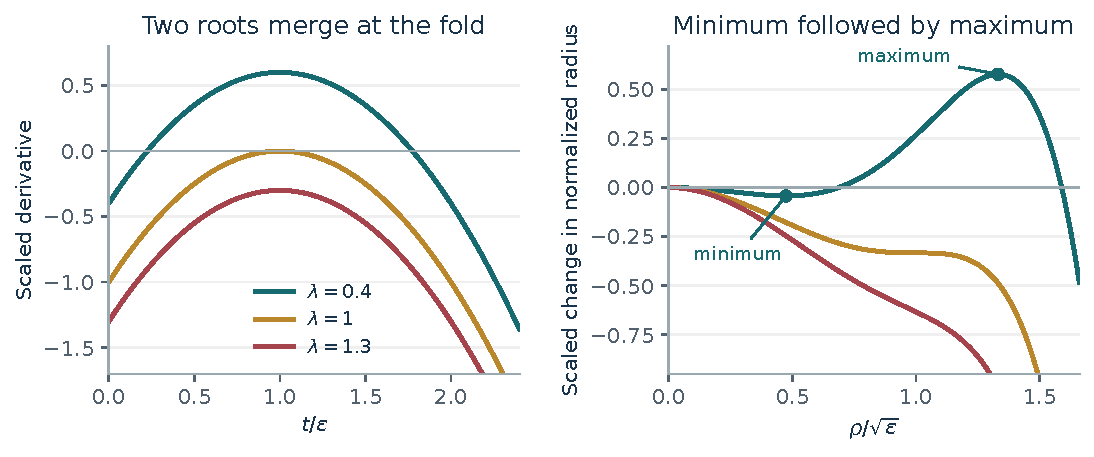
\includegraphics[width=\linewidth]{figures/radial_local_model.pdf}
\caption{The limiting local model on the paths
\eqref{turn:eq:scaling-path}. With $z=t/\varepsilon$ and
$u=\rho/\sqrt\varepsilon$, the scaled derivative is
$-\lambda+2z-z^2$ and the scaled change of normalized radius is
$-\lambda u^2+u^4-u^6/3$. The latter uses the positive scale
$-3R_0\varepsilon^3$. These are the proved leading local terms,
not direct numerical evaluations of the full function. The exact
fold has higher-order corrections to the displayed $\lambda=1$ model.}
\label{turn:fig:model}
\end{figure}

\subsection{What the result resolves and what remains}
\label{turn:sec:status}

The manuscript's displayed quartic-transition location is now replaced
by an exact rational enclosure, a local uniqueness theorem, a
transversality sign, and a negative sextic coefficient.  Its request
for the local higher-order radial behavior at that transition is
answered by Theorem~\ref{turn:thm:fold}.  The resulting region with a
minimum followed by a maximum is stronger than the preceding
existence results for one minimum or one maximum separately.

Three natural questions remain distinct.  First, is this the only
zero of $Q(a_*(b),b)$ in $0<b<1$?  Second, can one give explicit
numerical lower bounds for the parameter neighborhood and the fixed
radius $\sqrt T$ in the fold theorem?  Third, do the same parameter
pairs have additional turning points at larger radii?  The present
finite certificate answers none of these global or quantitative
questions by itself.  It establishes a nondegenerate local mechanism
that any proposed global classification must accommodate.

Another useful direction is the fully constant point $(a,b)=(1,1)$,
where $F_{1,1}(z)=\tfrac12\log^2(1-z)$ and
$\eta_{1,1}(\rho)=1/2$.  At that point every nonconstant radial
coefficient vanishes.  Relating that higher degeneracy to the nearby
certified fold requires further analysis; it cannot be inferred from
the sign of $R_0$ alone.  Proposition~\ref{turn:prop:recurrence}
provides an exact finite calculation at each order for such an
investigation.

\section{A constructive normal form for the full Cayley shuffle ideal}
\label{cay:sec:projection}

The earlier Cayley report determines the dimensions of two formal
presentations: the span of the unmultiplied Cayley rows, and the larger
shuffle ideal generated by them.  Its weight-seven search notes identify
an explicit reconstruction map for the latter quotient as a missing
computational step.  We provide such a map in every weight.  It gives
exact representatives without a relation matrix and produces a concrete
obstruction for the frozen $S_6$ formula after \emph{all} shuffle multiples
of Cayley identities have been included.

The shuffle-polynomial theorem and Eulerian idempotents used below are
classical \cite{cay:Radford,cay:Patras}.  The contribution to the inspected
project is the compatible endpoint projection, its combination with
those tools, the explicit reconstruction formula, and the resulting
weight-seven certificate.  Neither a period-independence assertion nor
the conjectured $S_6$ equality is established here.

\subsection{The algebra and its precise relation ideal}

Use the outer-letter-first convention and the five letters
\[
 z=\frac{dt}{t},\quad c=\frac{dt}{1-t},\quad
 a=\frac{i\,dt}{1-it},\quad b=-\frac{dt}{1+t},\quad
 \bar a=-\frac{i\,dt}{1+it}.
\]
Let $\widetilde{\mathcal A}$ be the rational shuffle algebra on these
letters, with empty word $1$ and shuffle product $\mathbin{\sqcup\!\sqcup}$.
Write $\mathcal A$ for its subalgebra spanned by $1$ and all words with
first letter different from $c$ and last letter different from $z$.
For such a word $w$, $H(w)$ is its convergent iterated integral from
zero to one.  Products written inside a word are concatenations unless
the shuffle symbol is displayed.

The Cayley involution is
\[
 C(v_1\cdots v_n)=\tau(v_n)\cdots\tau(v_1),\qquad
 \begin{array}{c|ccccc}
 v&z&c&a&b&\bar a\\ \hline
 \tau(v)&c-b&z+b&b-\bar a&b&b-a .
 \end{array}
\]
It preserves $\mathcal A$, is an automorphism for the shuffle product,
and commutes with the conjugation $K$ that exchanges $a,\bar a$ and
fixes $z,c,b$.  The change of variable $t\mapsto(1-t)/(1+t)$ proves
$H(Cw)=H(w)$ for admissible $w$.  Define
\begin{equation}\label{cay:eq:ideal}
 \mathcal J=\langle f-Cf:f\in\mathcal A\rangle_{\mathrm{shuffle}}.
\end{equation}
Thus $\mathcal J$ includes arbitrary products of convergent Cayley
relations with admissible words.  No stuffle, distribution, or other
functional equation is imposed in this definition.

\subsection{Endpoint projection that commutes with Cayley symmetry}

The ordinary projection that sets the divergent shuffle generators
$z,c$ to zero is unsuitable: it does not commute with $C$.  For example,
the ordinary projection of $Cz=c-b$ is $-b$, whereas $C$ applied to
the projection of $z$ is zero.  The needed correction is small but
essential.  Put
\begin{equation}\label{cay:eq:shifted-endpoints}
 x=z+\frac b2,\qquad y=c-\frac b2.
\end{equation}
Then $Cx=y$, $Cy=x$, and $Kx=x$, $Ky=y$.

\begin{lemma}[Equivariant endpoint projection]\label{cay:lem:regularization}
There is a unique shuffle-algebra retraction
$\mathcal R:\widetilde{\mathcal A}\to\mathcal A$ that is the identity
on $\mathcal A$ and sends $x,y$ to zero.  It commutes with $C,K$.
Equivalently, it substitutes $z=-b/2$, $c=b/2$ in
\emph{shuffle-polynomial coordinates}.

For a word $w$ of length $n$, let $l$ be its initial run of $c$'s and
$r$ its terminal run of $z$'s.  If $w[u:n-v]$ denotes deletion of
$u$ initial letters and $v$ terminal letters, then
\begin{equation}\label{cay:eq:regularization}
 \mathcal R(w)=
 \sum_{u=0}^{l}\sum_{v=0}^{r}
  \left(\frac b2-c\right)^u
  \mathbin{\sqcup\!\sqcup} w[u:n-v]
  \mathbin{\sqcup\!\sqcup}
  \left(-\frac b2-z\right)^v.
\end{equation}
The powers in this formula are concatenation powers of linear forms.
\end{lemma}

\begin{proof}
Order the alphabet as $z<a<b<\bar a<c$.  Every Lyndon word of length
at least two is admissible.  The shuffle-polynomial theorem
\cite{cay:Radford} and the
triangular Lyndon factorization therefore give
$\widetilde{\mathcal A}=\mathcal A[z,c]=\mathcal A[x,y]$ as polynomial
algebras.  Setting $x,y$ to zero defines the claimed retraction.  The
ideal $(x,y)$ is stable under both $C,K$, and both automorphisms preserve
$\mathcal A$; hence the retraction commutes with them.

For the formula, deletion of one initial $c$ and deletion of one terminal
$z$ are commuting derivations of the shuffle algebra.  Their Taylor
substitutions replace $c$ by $b/2$ and $z$ by $-b/2$.  The $u$th shuffle
power of a single linear form is $u!$ times its concatenation power,
which cancels the Taylor factorial.  This yields
\eqref{cay:eq:regularization}.  In particular every term left after
cancellation is admissible; this also follows from the range of the
retraction.
\end{proof}

This is a formal polynomial projection.  No value is assigned to a
divergent iterated integral, and no regularized analytic identity is
being assumed.  For example,
\[
 \mathcal R(az)=-za-\frac{ba+ab}{2},\qquad
 \mathcal R(c)=\frac b2,\qquad \mathcal R(z)=-\frac b2.
\]
The first formula also illustrates why a literal letter substitution
inside concatenation words would be incorrect.

\subsection{Explicit eigenvector lifts and the normal-form theorem}

For a nonempty word $w$, define the first Eulerian operator by
\begin{equation}\label{cay:eq:eulerian}
 e(w)=\sum_{k=1}^{|w|}\frac{(-1)^{k-1}}{k}
 \sum_{\substack{w=w_1\cdots w_k\\ |w_j|>0}}
  w_1\mathbin{\sqcup\!\sqcup}\cdots
  \mathbin{\sqcup\!\sqcup}w_k,\qquad e(1)=0.
\end{equation}
The inner sum is over consecutive nonempty blocks.  This is the
convolution logarithm of the identity for shuffle multiplication and
deconcatenation.  It annihilates a shuffle product of two positive-weight
elements and satisfies
\begin{equation}\label{cay:eq:eulerian-properties}
 e^2=e,\qquad e(f)-f\in
   (\widetilde{\mathcal A}_{>0})^2
 \quad(f\in\widetilde{\mathcal A}_{>0}).
\end{equation}
These are the standard Eulerian-idempotent properties in a connected
commutative Hopf algebra \cite{cay:Patras}.  The congruence is immediate
from \eqref{cay:eq:eulerian}; together with annihilation of products it
also proves the displayed idempotence.  Reversing the consecutive blocks
and using commutativity of shuffle shows directly that $e$ commutes
with $C$; it also commutes with $K$.

Set
\begin{equation}\label{cay:eq:lifts}
 E=\mathcal R e,\qquad
 E_+(w)=\frac{E(w)+C E(w)}2.
\end{equation}
All values of $E,E_+$ are admissible word polynomials.  The following
formula contains only finite sums of explicitly given rational words.

\begin{theorem}[Constructive full-ideal projector]\label{cay:thm:projector}
Define $\Pi(1)=1$ and, for every nonempty word,
\begin{equation}\label{cay:eq:projection}
 \boxed{\displaystyle
 \Pi(w)=\sum_{k=1}^{|w|}\frac1{k!}
   \sum_{\substack{w=w_1\cdots w_k\\ |w_j|>0}}
    E_+(w_1)\mathbin{\sqcup\!\sqcup}\cdots
     \mathbin{\sqcup\!\sqcup}E_+(w_k).}
\end{equation}
Then $\Pi:\widetilde{\mathcal A}\to\mathcal A$ is a graded
shuffle-algebra homomorphism.  Its restriction to $\mathcal A$ satisfies
\begin{equation}\label{cay:eq:projection-properties}
 \Pi^2=\Pi,\qquad \Pi C=C\Pi=\Pi,\qquad \Pi K=K\Pi,
 \qquad \ker(\Pi|_{\mathcal A})=\mathcal J.
\end{equation}
Consequently $\Pi(f)=\Pi(g)$ if and only if $f-g\in\mathcal J$ for
$f,g\in\mathcal A$.  In particular, every admissible word has the
proved period identity
\begin{equation}\label{cay:eq:period-normal-form}
 H(w)=H(\Pi(w)).
\end{equation}
\end{theorem}

\begin{proof}
First restrict $E$ to $\mathcal A$.  It annihilates products of two
positive-weight elements, and $E(f)-f\in(\mathcal A_{>0})^2$ because
$\mathcal R$ preserves products and positive degree.  Hence $E^2=E$
on $\mathcal A$, and its image $U=E(\mathcal A)$ maps isomorphically to
the indecomposables
$\mathcal A_{>0}/(\mathcal A_{>0})^2$.  Lifts of any homogeneous basis
of those indecomposables freely generate the polynomial algebra
$\mathcal A$: the change from its Lyndon generators is degree triangular
with invertible linear part.  Thus multiplication gives an isomorphism
$\operatorname{Sym}(U)\simeq\mathcal A$.

Since $\mathcal R,e$ commute with $C,K$, the space $U$ is stable under
both.  Write $U=U_+\oplus U_-$ for its $C$ eigenspaces.  The algebra
map that fixes $U_+$ and kills $U_-$ is an idempotent map $P$ on
$\mathcal A$.  Its kernel is the ideal generated by $U_-$.  This ideal
equals $\mathcal J$: if $u\in U_-$, then $u-Cu=2u$; conversely $C$
acts as the identity after the negative generators have been killed,
so every $f-Cf$ belongs to that ideal.  The map $P$ commutes with $K$.

It remains to verify that the fully explicit formula is this map.
For every nonempty $w$, convolution exponentiation gives
\[
 w=\sum_{k=1}^{|w|}\frac1{k!}
   \sum_{w=w_1\cdots w_k}
    e(w_1)\mathbin{\sqcup\!\sqcup}\cdots
     \mathbin{\sqcup\!\sqcup}e(w_k).
\]
Applying $\mathcal R$ gives the same formula for $\mathcal R(w)$
with factors $E(w_j)$.  Those factors belong to $U$, including when
the blocks themselves are not admissible.  To see this last point,
write $\widetilde{\mathcal A}=\mathcal A[x,y]$.  In degree at least
two, every term of $w-\mathcal R(w)$ that involves $x$ or $y$ is a
product of positive-degree factors and is annihilated by $e$; in degree
one, applying $\mathcal R e$ kills $x,y$ directly.  Thus
$E(w)=E(\mathcal R(w))\in U$ in every degree.

Now apply the algebra map $P$.  On $U$, it acts by $(1+C)/2$, so the
result is exactly \eqref{cay:eq:projection}.  Therefore
$\Pi=P\mathcal R$, proving multiplicativity and every assertion in
\eqref{cay:eq:projection-properties}.  Finally, $w-\Pi(w)\in\mathcal J$
for admissible $w$.  The map $H$ annihilates this ideal by the convergent
Cayley identity and the shuffle product law, proving
\eqref{cay:eq:period-normal-form}.
\end{proof}

For example, the three admissible weight-one letters give
\[
 \Pi(a)=\frac{a+b-\bar a}{2},\qquad
 \Pi(\bar a)=\frac{\bar a+b-a}{2},\qquad \Pi(b)=b.
\]
Evaluating the first identity recovers
$\Li_1(i)+\Li_1(-i)=\Li_1(-1)$, including its sign.  At higher weights
the projector automatically includes the products of the corresponding
Cayley-negative generators, which the raw average $(1+C)/2$ does not
annihilate.  The image is the same quotient whose weight-seven imaginary
dimension was previously proved to be $7518$.  Formula
\eqref{cay:eq:projection} supplies representatives in the original word
coordinates; it does not claim that the resulting sparse supports are
already a chosen $7518$-element basis.

\subsection{An exact obstruction for the frozen weight-seven target}

The series convention is
$\Li_{r,s}(u,v)=\sum_{n>m\ge1}u^nv^m/(n^rm^s)$.  Consequently
\[
 H(z^{r-1}a z^{s-1}a)=\Li_{r,s}(i,1),\qquad
 H(z^5a\bar a)=\Li_{6,1}(i,-1).
\]
Here $G=\beta(2)$ is Catalan's constant, and
\[
 S_6=\sum_{n=0}^{\infty}\frac{(-1)^nH_n}{(2n+1)^6},\qquad
 H_n=\sum_{j=1}^{n}\frac1j,\qquad H_0=0,
 \quad g_{r,s}=\operatorname{Im}\Li_{r,s}(i,1).
\]
Let $F$ be the following explicitly fixed formal lift of the conjectured
integer relation:
\begin{align}
 F={}&-179712000z^5aa+485683200z^5a\bar a
       -36864000z^3az^2a+401080320zaz^4a\notag\\
 &-\frac{47600087040}{61}z^6a
       +11750400(za\mathbin{\sqcup\!\sqcup}z^4c)\notag\\
 &+109347840(z^3a\mathbin{\sqcup\!\sqcup}z^2c)
       -971366400(z^5a\mathbin{\sqcup\!\sqcup}b).
 \label{cay:eq:target}
\end{align}
Indeed $\beta(7)=61\pi^7/184320$, $\Li_1(-1)=-\log2$, and the
harmonic parity split gives
\begin{align*}
 \operatorname{Im}H(F)={}&485683200S_6-665395200g_{6,1}
 -36864000g_{4,3}+401080320g_{2,5}\\
 &-258247\pi^7+11750400G\zeta(5)
 +109347840\beta(4)\zeta(3)+971366400\beta(6)\log2.
\end{align*}

For a word polynomial $f$, define its imaginary coordinate reduction
$\mathcal O(f)$ by replacing each conjugate pair $w,Kw$ by
$(f_w-f_{Kw})w$, choosing the lexicographically smaller representative
under the code order $z<c<a<b<\bar a$; conjugation-fixed words are
discarded.  This convention encodes imaginary parts without a factor
of $1/2$.

\begin{lemma}[An all-weight separating coordinate]\label{cay:lem:coordinate}
For an integer $w\ge3$, put
$\ell_w(f)=[z^{w-2}aa]\mathcal O(\Pi(f))$.
For positive integers $r,s$ with $r+s=w$,
\begin{equation}\label{cay:eq:coordinate-family}
 \ell_w(z^{r-1}az^{s-1}a)=\frac{\delta_{s,1}}4,
 \qquad
 \ell_w(z^{w-2}a\bar a)=-\frac14.
\end{equation}
Moreover $\ell_w$ vanishes on every word with at most one occurrence
of $a$ or $\bar a$.
\end{lemma}
\begin{proof}
Write $N=w-2>0$.  To contribute to $z^Naa$, a projected word on
$\{z,a,\bar a\}$ must retain every zero letter and both nonreal
letters.  A block consisting only of zero letters cannot do this:
its Eulerian image is zero if its length exceeds one, and
$\mathcal R(z)=-b/2$ otherwise.  Also $CE$ of any such block contains
no $z$, since $E$ introduces no $c$ and $\tau(z)=c-b$.
Thus only one-block and two-block terms of
\eqref{cay:eq:projection} can contribute, and each block containing
a zero letter must use the $E/2$ part of $E_+$.

For a block containing just one $a$, its component with all zeros
retained is the usual right-endpoint shuffle regularization
\[
 z^uaz^v\longmapsto
 (-1)^v\binom{u+v}{v}z^{u+v}a.
\]
Indeed setting the shuffle variable $z$ to zero kills every product
term in $e(z^uaz^v)-(z^uaz^v)$, because each such product has a
factor consisting only of zeros.  The displayed formula follows by
shuffle regularization, or by induction on $v$ using the shuffle
product with $z$.

For $z^{r-1}az^{s-1}a$, the sum of the two-block shuffle coefficients
at $z^Naa$ is therefore
\[
 \Sigma=2\sum_{j=0}^{s-1}(-1)^j
   \binom{r-1+j}{j}\binom{N}{r-1+j}
 =2\binom{N}{r-1}\sum_{j=0}^{s-1}(-1)^j\binom{s-1}{j}
 =2\delta_{s,1}.
\]
Convolution exponentiation before the Cayley projection says that
the one-block coefficient is $\delta_{s,1}-\Sigma/2$.
After projection, the one-block term is multiplied by $1/2$ and
the two-block sum by $1/8$.  Their total is
$\delta_{s,1}/2-\Sigma/8=\delta_{s,1}/4$.
There is no $z^N\bar a\bar a$ contribution: obtaining both
conjugate letters would require the $CE$ part of both blocks, and
at least one block contains a zero letter.

For $z^Na\bar a$, the only contributing cut is $z^Na\mid\bar a$.
The first factor contributes $z^Na/2$ and the second contributes
$-a/2$ from $C\bar a=b-a$.  The exponential factor $1/2!$ and
the coefficient $2$ of $z^Naa$ in $z^Na\mathbin{\sqcup\!\sqcup}a$
give $-1/4$.  Again the conjugate coordinate is absent.  Finally,
$e,\mathcal R,C$ never increase the number of nonreal letters.
Every term of \eqref{cay:eq:projection} consequently has at most
one such letter when the original word does, proving the last assertion.
\end{proof}

\begin{proposition}[Full Cayley-ideal separation]\label{cay:prop:separation}
The rational functional
\[
 \ell(f)=[z^5aa]\,\mathcal O(\Pi(f))
\]
annihilates the full ideal $\mathcal J$ and satisfies
\begin{equation}\label{cay:eq:separation}
 \ell(F)=-166348800\ne0.
\end{equation}
Thus the imaginary lift of the frozen target is not a consequence of
convergent Cayley symmetry and its complete shuffle-multiplicative
closure.
\end{proposition}

\begin{proof}
Annihilation follows from Theorem~\ref{cay:thm:projector}.
Lemma~\ref{cay:lem:coordinate} gives
\[
\begin{array}{c|ccccc}
 f&z^5aa&z^5a\bar a&z^3az^2a&zaz^4a&z^6a\\ \hline
 \ell(f)&1/4&-1/4&0&0&0 .
\end{array}
\]
Each word in the three shuffle products in \eqref{cay:eq:target}
has just one nonreal letter, so those products also have value zero
under $\ell$.  The table gives
$(-179712000-485683200)/4=-166348800$.
The supplied program replays these exact rational calculations as
an independent finite audit of the analytic formula.
More explicitly, $\Pi$ commutes with $K$, so
$\mathcal O(\Pi(F))\ne0$ implies
$\Pi((F-KF)/2)\ne0$.  The kernel theorem therefore gives
$(F-KF)/2\notin\mathcal J$, which is the asserted imaginary statement.
\end{proof}

The complete $\mathcal O(\Pi(F))$ has $3444$ nonzero word coordinates;
it is provided as \src{data/cayley_s6_normal_form.json}.
The displayed nonzero coefficient alone is sufficient for separation.
This does not contradict the very small certified numerical residual
of $F$.  It proves nonmembership in a specified formal ideal whose
definition omits double shuffle and other available period identities.
In particular, the new certificate does not assert nonmembership in
the separate $5131$-row presentation, does not enlarge that row
presentation by implication, and does not establish or disprove the
numerical conjecture.

\subsection{Verification and the next reduction step}

The independent formulas exposed in the code are useful for auditing
the construction.  The implementation of $e$ uses the equivalent
permutation formula
\[
 e(v_1\cdots v_n)=\sum_{\sigma\in S_n}
 \frac{(-1)^{d(\sigma^{-1})}}
 {n\binom{n-1}{d(\sigma^{-1})}}
 v_{\sigma(1)}\cdots v_{\sigma(n)},
\]
where $d$ counts descents.  It follows directly from
\eqref{cay:eq:eulerian}: a permutation can arise from a cut into $k$
blocks exactly when the $k-1$ cut positions include every descent of
the inverse permutation.  Summing
$(-1)^{k-1}\binom{n-1-d}{k-1-d}/k$ gives the displayed coefficient.
The verifier compares this implementation with the consecutive-cut
definition on small distinct-letter words.  It also checks the
projection and product identities on all words and all shuffle products
of total weight at most four, then reconstructs the weight-seven target
and its separating values with rational arithmetic.

A combined proof search can now replace each additional exact
relation $R$ by $\Pi(R)$ and the target by $\Pi(F)$.  For any specified
family $\mathscr R\subset\mathcal A$, the elementary equivalence
\[
 F\in\mathcal J+\operatorname{span}_{\mathbb Q}\mathscr R
 \quad\Longleftrightarrow\quad
 \Pi(F)\in\operatorname{span}_{\mathbb Q}\{\Pi(R):R\in\mathscr R\}
\]
follows by subtracting $f-\Pi(f)\in\mathcal J$.
This supplies an exact, reconstructible way to impose the full
Cayley ideal before searching the additional double-shuffle rows.
It is a completed reduction tool for that next search, rather than a
claim that the remaining search has already succeeded.

\section{Manuscript updates and a further research program}
\label{sec:agenda}

The four parts of this article have different mathematical outputs.
The Euler theorem proves a uniform inequality and identifies its exact
optimal constant. The golden certificates prove special-value and
functional identities. The radial theorem classifies a local change
in the shape of a zero curve. The Cayley theorem constructs an
algebraic quotient and separates a target from a specific relation
ideal. Their common feature is that each conclusion has a finite,
explicit point of verification, together with an analytic or algebraic
argument explaining why that verification suffices.

\subsection{Corrections of status and scope}

No false displayed formula was established in the source material
audited for this continuation. The proposed corrections are therefore
specific updates of proof status and precise limitations on how the
new results may be used. A blanket assertion that the entire
375-page manuscript has been verified would exceed this audit.

\paragraph{The universal Euler question is settled.}
The question in \src{chapters/10-discovery.tex} asking for a universal
real-order Euler bound above the critical triangle can be replaced by
\cref{eul:thm:main}. Its earlier parameter-dependent bounds remain valid
and can still be useful when they are smaller. The new result provides
the universal budget $9/(8\,2^N)$ for $N\ge2$ and identifies the optimal
constant for all $N\ge1$. The exact critical-triangle constant also
remains a separate sharper statement on its restricted parameter set.

The source's warning that the Gaussian maximum alone does not furnish
the universal Euler bound is mathematically correct. It should be
retained as an explanation of the missing implication, followed by the
new positive-tail representation and uniform kernel gap. The proof
cannot be shortened by deleting that step. In particular, a bound on
the complete sum does not automatically bound every rescaled tail.

\paragraph{The remaining displayed golden weight-five formulas are proved.}
The numerical-evidence paragraph preceding the second and third
weight-five formulas in \src{chapters/03-algebraic.tex} can now cite
\cref{gold:thm:main}. The canonical index-$12$, $20$, and $24$
normalizations and their lower-weight vanishing statements can be
updated using the exact descent and recombination in
\cref{gold:sec}. The earlier numerical checks are useful historical
evidence but are no longer the justification for these identities.

The weight-$6$ through weight-$9$ formulas retain their prior
conjectural status. Contracting a weight-five tensor proves identities
of lower weight; it cannot create a weight-six tensor identity.
Likewise, a successful finite alphabet does not prove that its
specializations exhaust all numerical relations at the golden ratio.

\paragraph{The quartic-transition question has a local answer.}
The decimal transition in \src{chapters/05-real-turning.tex} can be
supplemented by the exact rational rectangle in
\cref{turn:thm:transition}. The higher radial behavior is given by the
negative sextic coefficient and \cref{turn:thm:fold}. There is exactly
one transition in the stated rectangle, and an open local region with
two small-radius turning points. Neither assertion proves that this is
the only transition on the entire threshold curve or that these are
the only turning points in the full disk.

\paragraph{The Cayley obstruction is strengthened, while $S_6$ stays open.}
The projector in \cref{cay:thm:projector} supplies a constructive
normal form for the full ideal of convergent Cayley relations and
their shuffle multiples. The exact separating coordinate applies to
that whole ideal. It is stronger than a failure to solve one bounded
matrix system, but still concerns a specified formal presentation.
The conjectural numerical equality for $S_6$ could be proved by
relations that are absent from this ideal. Its $S_8$ analogue is also
untouched. A nonzero formal normal form must not be reported as a
nonzero special value.

\paragraph{Two bookkeeping rules should accompany integration.}
First, rational constant factors in $1-f$ belong to the golden tensor
calculation: the factor $2$ in $1-(1-t)/(1+t)$ is a simple example.
Removing all constant factors would remove logarithmic information.
Second, Cayley-compatible endpoint projection must use the shifted
generators $z+b/2$ and $c-b/2$. Setting the unshifted endpoint
generators to zero does not commute with the involution. These are
requirements of the new proofs, not allegations that the baseline
already made either mistake.

The accompanying \src{integration/INTEGRATION.md} gives concrete
source locations, replacement prose, and the label mapping. All
integration should be compared with the pinned baseline: later
repository changes may already incorporate some of these statements.

\subsection{Research questions on uniform bounds and asymptotics}

\paragraph{1. Optimize the later Euler steps.}
For each integer $N\ge2$, define
\[
 C_N^{\mathrm{av}}=
 \sup_{a,b>0}\E[\mathcal K_N(X_a,Y_b)],\qquad
 C_N^{\mathrm{pt}}=
 \max_{0\le x,y\le1}\mathcal K_N(x,y),
\]
where the boundary value at $y=1$ is continuous. The present theorem
gives $C_N^{\mathrm{av}}\le C_N^{\mathrm{pt}}<9/8$. Determine either
sequence sharply. The two optimization problems should be kept
separate: the gamma laws form a restricted family of probability
measures, so a pointwise maximizer need not be approachable by these
averages. A useful first target is an exact algebraic description of
the pointwise maximum for $N=2$, obtained from its rational stationary
equations and certified boundary comparisons.

\paragraph{2. Determine the fixed-parameter tail asymptotics.}
For fixed $a,b>0$, the exact kernel representation suggests a sharper
description than a universal constant times $2^{-N}$. The transition
of $(1-x^2y^2)^N$ occurs near $xy\asymp N^{-1/2}$. The product
$XY$ has $-\log(XY)$ gamma distributed with shape $a+b$, so Mellin
analysis of that region is natural. The difficulty is to retain the
cancellation in $(W_N(xy)-W_N(x))/(1-y)$ uniformly near $y=1$.
A proof should state its leading term and remainder uniformly on
compact positive parameter sets, then study what fails as an order
approaches zero. This could give much smaller parameter-sensitive
error budgets without weakening the unconditional universal bound.

\paragraph{3. Extend the positive-tail method to other arguments.}
At the Gaussian point, the alternating series and the rational
denominators align particularly well. Which roots of unity, or which
fixed angles in the slit plane, admit a transform whose remainder is
a positive probability average? The first concrete experiment should
be a residue-class decomposition at a primitive sixth root. A useful
theorem would identify the angle-dependent kernel and its sign before
attempting a global numerical constant. At a general angle, positivity
may fail even though the analytic continuation remains well defined.

\subsection{Research questions on radial geometry}

\paragraph{4. Prove or refute global uniqueness of the quartic transition.}
The precise unresolved assertion is that
$Q(a_*(b),b)=0$ has only the certified solution for $0<b<1$.
The determinant calculation already provides a positive derivative
along the threshold in a small neighborhood. An effective program
would combine analytic endpoint expansions at $b\downarrow0$ and
$b\uparrow1$ with a finite interval covering of the remaining compact
interval. A plot of the threshold is not sufficient, especially near
the fully constant point $(1,1)$, where several coefficients vanish.

\paragraph{5. Make the double-turning neighborhood effective.}
The local theorem proves the existence of a fixed radius and a
parameter neighborhood but does not print their sizes. One can seek
explicit bounds for $U_{tt}$ and the fourth and higher Taylor
remainders on a rational parameter box and $0\le t\le T$. The
all-orders recurrence isolates each coefficient, while a Cauchy bound
on the normalized implicit equation can control the infinite tail.
The resulting certificate should exhibit actual rational parameter
pairs with two certified turning-radius intervals. This is a natural
next strengthening of the current existence theorem.

\paragraph{6. Understand the all-orders degeneracy at $(1,1)$.}
At that point $F_{1,1}(z)=\tfrac12\log^2(1-z)$ and the normalized
radius is identically $1/2$. The nearby double-turning transition has
a nonzero sextic coefficient. Determine the first-order parameter
variation of the entire function $\Phi$, rather than one Taylor
coefficient at a time, and ask whether it constrains the number of
small-radius oscillations. This may clarify the relationship between
the isolated certified transition and the infinitely degenerate
constant curve. It must also be reconciled with the still-open
full-radius motion conjectures for integer outer order.

\subsection{Research questions on identities and relation spaces}

\paragraph{7. Lift the golden weight-six and weight-seven candidates.}
The two higher reconstructions in the manuscript are concrete next
targets. Search for a rational-function tensor certificate of the
correct weight whose specialization is exactly the proposed vector,
including its logarithmic completion. Gangl's work
\cite{Gangl} gives relevant higher-weight functional identities and
uses richer multiplicative alphabets. A search restricted to
$t,1-t,1+t$ should therefore be treated as one finite model. The
essential deliverables are an exact tensor row, an endpoint constant,
and ordinary-polylogarithm reconstruction, not only a nullspace rank.
The weight-eight and weight-nine formulas require a further step and
should not be assumed to follow once weights six and seven are solved.

\paragraph{8. Simplify and classify the functional certificates.}
Can the $58$- and $60$-term rows be expressed as short combinations of
classical Kummer specializations? Such a decomposition could reveal
why the golden specialization eliminates the unwanted powers. A
separate finite problem is to determine the exact image of the full
degree-bounded tensor kernel under golden specialization. Its rank
and nullspace can be certified by rational linear algebra. Any
minimality result must explicitly retain the alphabet and degree
bound; it would not establish independence of the resulting periods.

\paragraph{9. Specialize the new functional identities in other fields.}
The identities \eqref{gold:eq:new-functional-identities} hold for all
$0<t<1$, so their use is not confined to the golden ratio. For
example, with $\sigma=\sqrt2-1$, one has
$1-\sigma=\sqrt2\,\sigma$ and $1+\sigma=\sqrt2$. Every table argument
then becomes
\[
 s\,\sigma^{a+b}2^{(b+c)/2}.
\]
Substitution gives two exact weight-five relations in
$\mathbb Q(\sqrt2)$ with the same displayed endpoint constants.
The research problem is to combine them with duplication, inversion,
and other field relations until a small useful basis emerges. This
provides a structured source of new candidate evaluations. It avoids
guessing a large unrelated list of numerical constants at the outset.

\paragraph{10. Add the missing relations to the Cayley quotient.}
For a proposed collection of additional relation vectors
$\mathcal T$, the exact next computation is to ask whether
\[
 \Pi(F)\in\operatorname{span}_{\mathbb Q}\{\Pi(T):T\in\mathcal T\}.
\]
The equivalence with membership in the original Cayley ideal plus
these additional rows follows from the kernel theorem. Thus every
candidate stuffle, distribution, or complementary-argument identity
can be projected immediately. Start with convergent relations and
lower-weight products, then introduce regularized relations only with
their analytic conventions stated explicitly. The nonzero coordinate
$-166348800$ identifies information that the added relations must
actually supply. If the enlarged presentation still fails, report
that precise obstruction; it would not settle numerical independence.

\paragraph{11. Make the quotient computationally practical in higher weight.}
The explicit word projector is finite, but its expanded support grows
quickly. A representation by Cayley-positive Eulerian generators can
retain products in factored form and postpone full shuffle expansion.
Determine the cost of converting a specified target to these
coordinates, and compare it with elimination in a relation matrix.
A useful implementation should return a reconstruction certificate,
so that compression never hides the formal identity it represents.
The all-weight separating-coordinate lemma suggests that many target
tests may need only a few coordinates of the projector.

\paragraph{12. Formalize the smallest complete proof path.}
The Euler result offers a manageable entry point: polynomial
identities, rational Bernstein positivity, the probability-kernel
formula, and the truncated-power mixture. The golden result offers a
different path through finite tensor identities and one-variable
calculus. A proof-assistant project should first choose one complete
analytic theorem, rather than merely formalizing its arithmetic
receipt. In either case, the present records separate the finite
equalities from the mathematical implications they support.

\subsection{Reproduction and the boundary of the deliverable}

The archive is arranged so that the proofs and their finite premises
can be inspected independently. The article contains all definitions,
the golden coefficient tables, the three Euler polynomials, and the
local radial coefficient formulas. The data files contain the full
Bernstein partitions, the rational interval bounds, the exact golden
rows and their specialization receipts, and the Cayley normal form.
The independent review notes explain the delicate analytic and
algebraic steps.

From the extracted directory, the commands
\begin{verbatim}
python3 -m pip install -r requirements.txt
python3 code/run_all.py
latexmk -pdf -interaction=nonstopmode -halt-on-error article.tex
\end{verbatim}
replay the certificates and rebuild the article. The requirements file
lists the Python dependencies used for replay and figure generation;
the two core Euler and radial producers use only Python's standard
library. The golden verifier and independent Euler reviewer use SymPy
for exact symbolic arithmetic. The Cayley verifier uses rational
arithmetic throughout. Figure generation is optional and is invoked
by adding \texttt{--figures} to the replay command.

No integer-relation search is needed to verify the accepted golden
identities, and no numerical root solver is needed to certify the
radial rectangle. The figures visualize the proved structure and are
explicitly labeled as diagnostic or as a limiting local model. The
open questions above remain open in this deliverable; they are not
silently promoted by successful numerical comparisons or by the
strength of a neighboring theorem.

\begin{thebibliography}{99}
\addcontentsline{toc}{section}{References}

\bibitem{Repo}
V.~Reshetnikov and contributors,
\emph{Polylogarithms and their Arithmetic Bridges}, ProveIt repository,
\src{Analysis/Polylogarithms/docs/manuscript}, revision
\baseline, audited 10 October 2026.
\url{https://github.com/VladimirReshetnikov/ProveIt/tree/3447bc59b78d138a7f0d536b66ac6e5cc5d5e49f/Analysis/Polylogarithms/docs/manuscript}.
The specific source files and proposed integration locations are listed
in \src{integration/INTEGRATION.md}.

\bibitem{DLMFeuler}
NIST Digital Library of Mathematical Functions,
\S3.9, \emph{Acceleration of Convergence}, especially
\S3.9(ii), Euler's transformation of series.
\url{https://dlmf.nist.gov/3.9}.

\bibitem{Williamson}
R.~E. Williamson,
\emph{Multiply monotone functions and their Laplace transforms},
Duke Mathematical Journal \textbf{23} (1956), no.~2, 189--207.
\href{https://doi.org/10.1215/S0012-7094-56-02317-1}{doi:10.1215/S0012-7094-56-02317-1}.

\bibitem{McNeilNeslehova}
A.~J. McNeil and J.~Ne\v{s}lehov\'a,
\emph{Multivariate Archimedean copulas, $d$-monotone functions and
$\ell_1$-norm symmetric distributions},
The Annals of Statistics \textbf{37} (2009), no.~5B, 3059--3097.
\href{https://doi.org/10.1214/07-AOS556}{doi:10.1214/07-AOS556}.
\url{https://arxiv.org/abs/0908.3750}.

\bibitem{AbouzahraLewin}
M.~Abouzahra and L.~Lewin,
\emph{The polylogarithm in algebraic number fields},
Journal of Number Theory \textbf{21} (1985), no.~2, 214--244.
\href{https://doi.org/10.1016/0022-314X(85)90052-6}{doi:10.1016/0022-314X(85)90052-6}.

\bibitem{Gangl}
H.~Gangl, \emph{Functional equations and ladders for polylogarithms},
Communications in Number Theory and Physics \textbf{7} (2013), no.~3,
397--410.
\href{https://doi.org/10.4310/CNTP.2013.v7.n3.a1}{doi:10.4310/CNTP.2013.v7.n3.a1}.
Author manuscript:
\url{https://www.maths.dur.ac.uk/users/herbert.gangl/ladders1_ams.pdf}.

\bibitem{cay:Radford}
D.~E. Radford,
\emph{A natural ring basis for the shuffle algebra and an application
to group schemes}, Journal of Algebra \textbf{58} (1979), no.~2,
432--454.
\href{https://doi.org/10.1016/0021-8693(79)90171-6}{doi:10.1016/0021-8693(79)90171-6}.

\bibitem{cay:Patras}
F.~Patras, \emph{La d\'ecomposition en poids des alg\`ebres de Hopf},
Annales de l'Institut Fourier \textbf{43} (1993), no.~4, 1067--1087.
\href{https://doi.org/10.5802/aif.1365}{doi:10.5802/aif.1365}.
\url{https://www.numdam.org/item/AIF_1993__43_4_1067_0/}.

\end{thebibliography}

\end{document}
